\documentclass[aspectratio=169]{beamer}

\usetheme[progressbar=frametitle]{metropolis}
\usepackage{appendixnumberbeamer}
\usepackage{booktabs}
\usepackage[scale=2]{ccicons}
\usepackage{xspace}
\usepackage{caption}
\usepackage{subcaption}
\usepackage{amsmath, amssymb}

\title{Лекция 1: Введение в AI}
\subtitle{История вопроса и причём тут машинное обучение}
\date{23 января 2021}

\begin{document}

\maketitle

\begin{frame}{Кто такие нейросети и где они живут}
    \centering
    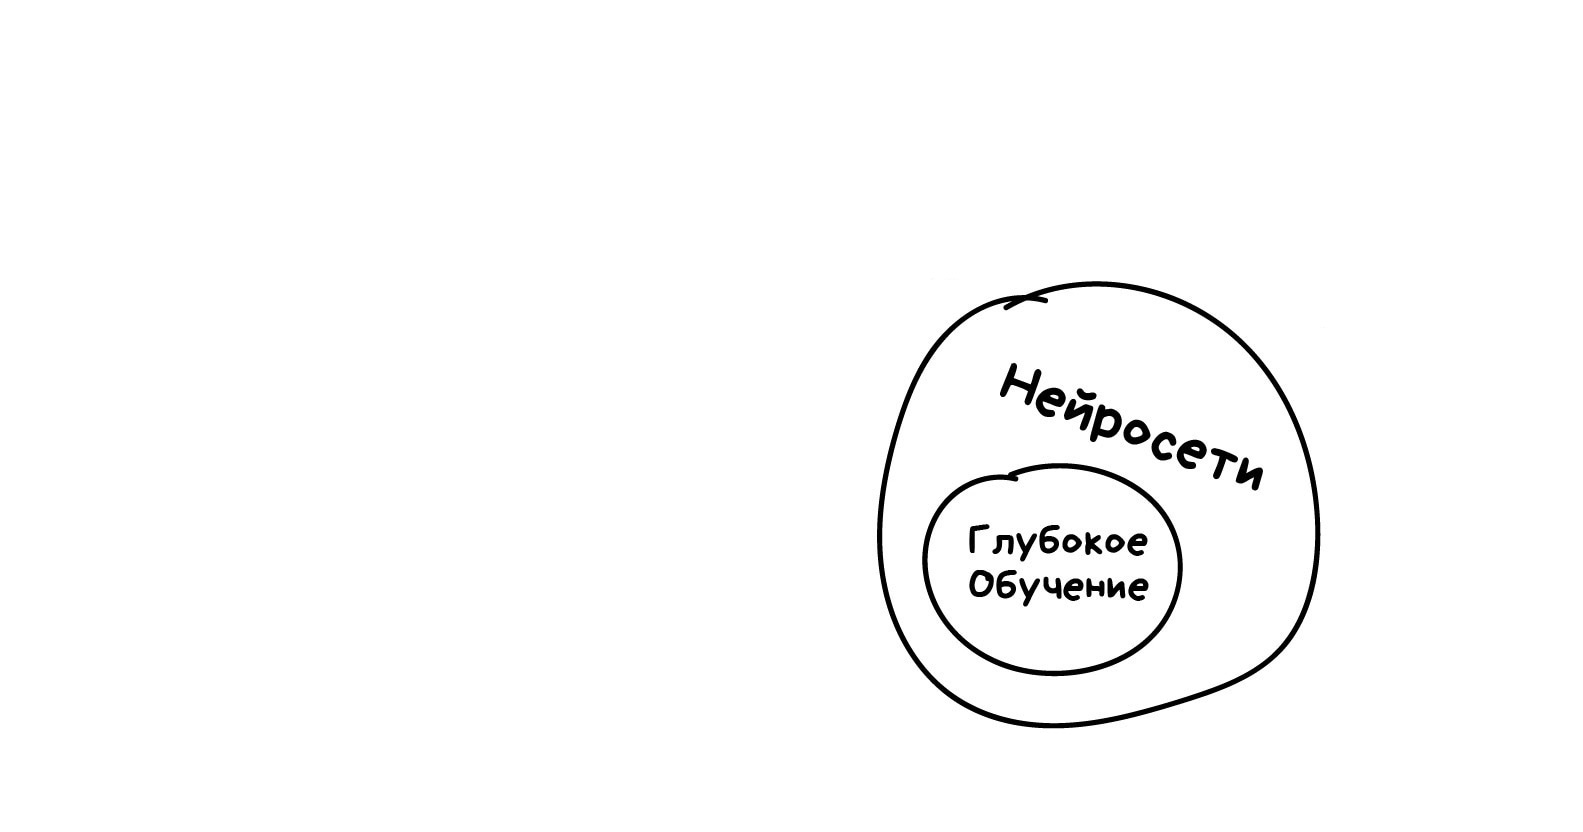
\includegraphics[width=.9\linewidth]{graphs/fig1_0.jpg}
\end{frame}

\begin{frame}{Кто такие нейросети и где они живут}
    \centering
    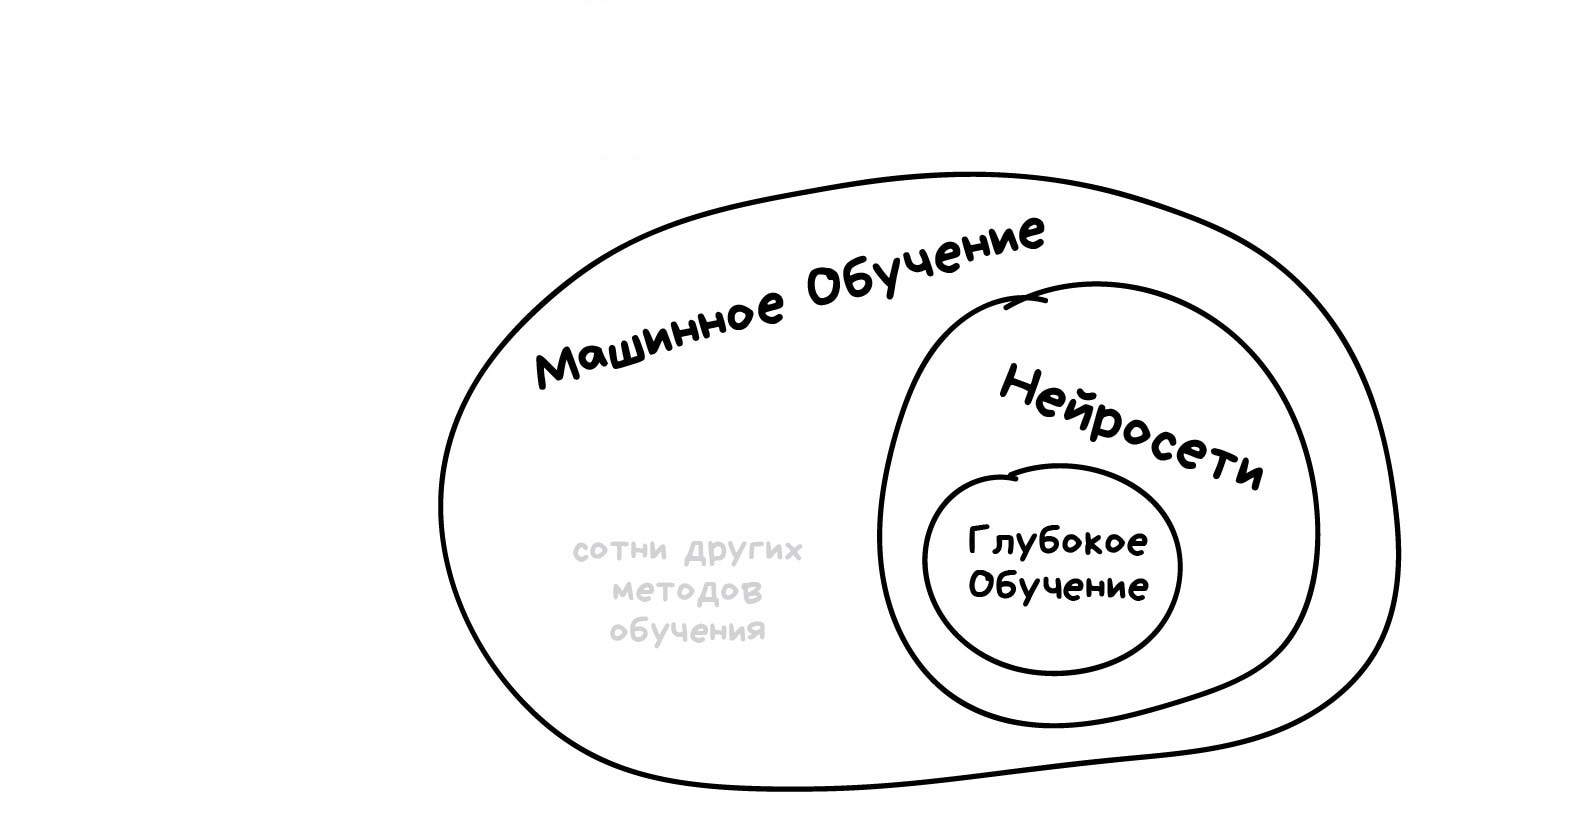
\includegraphics[width=.9\linewidth]{graphs/fig1_1.jpg}
\end{frame}

\begin{frame}{Кто такие нейросети и где они живут}
    \centering
    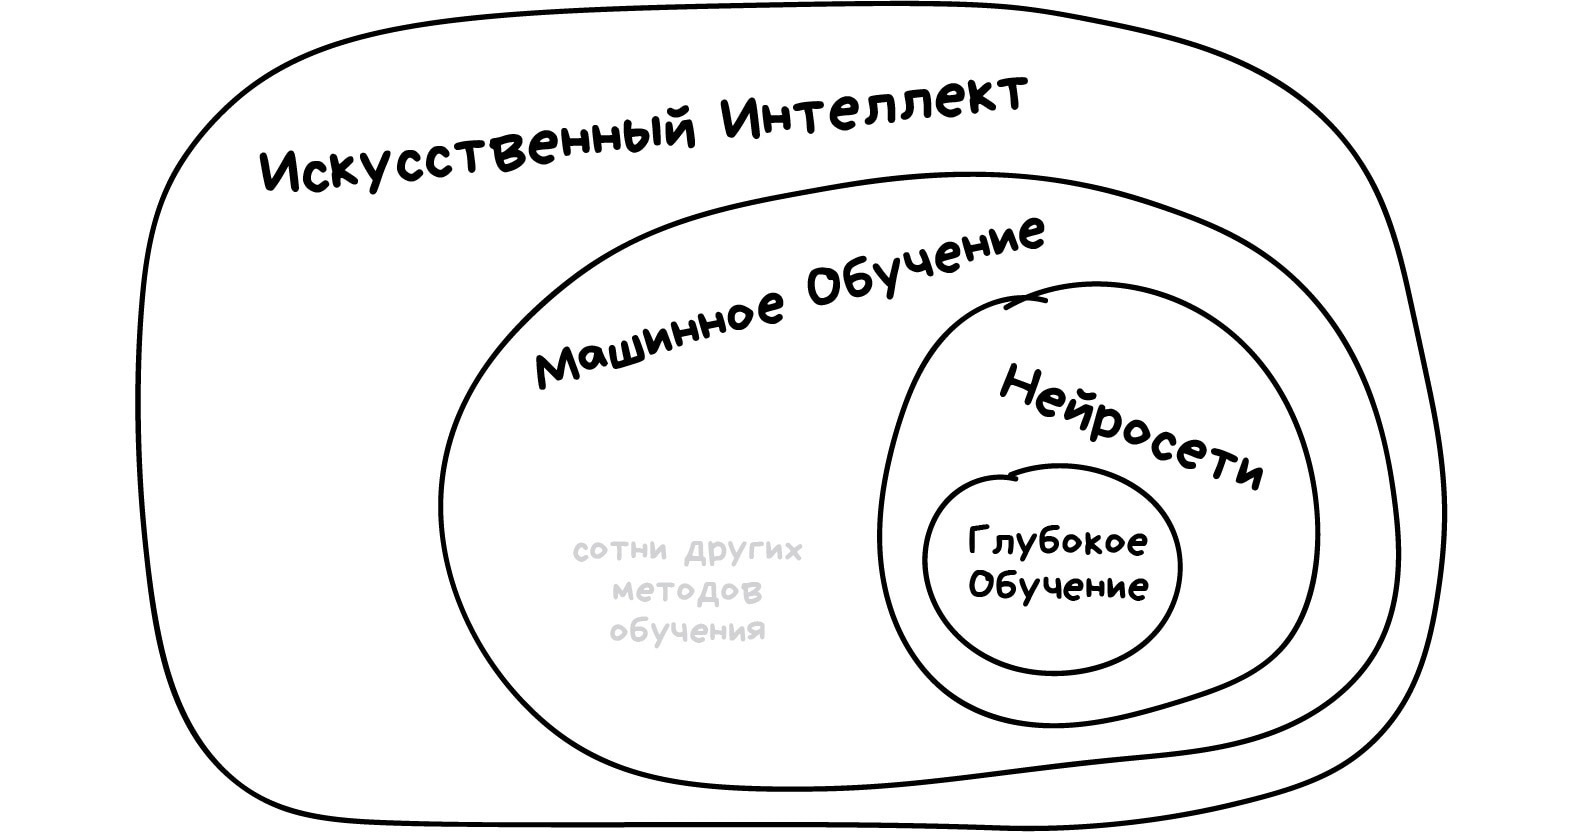
\includegraphics[width=.9\linewidth]{graphs/fig1_2.jpg}
\end{frame}

\begin{frame}{Область искусственного интеллекта}
    Исследования в области искусственного интеллекта --- научные исследования, ставящие
    своей целью построить вычислимые алгоритмы для решения ``когнитивных'' задач.\\
    \pause{}
    \textbf{Когнитивные} задачи --- задачи, которые человек обычно решает
    (или решал до недавнего времени) намного лучше программ, например:
    \begin{itemize}
        \item Перевод
        \item Распознавание речи, объектов
        \item Поиск ответов на нечетко сформулированные вопросы
        \item Интеллектуальные игры (шахматы, го, \ldots)
        \item Управление техникой (автомобилем, \ldots)
        \item \ldots
    \end{itemize}
\end{frame}

\begin{frame}{Хронология}
    \begin{figure}
        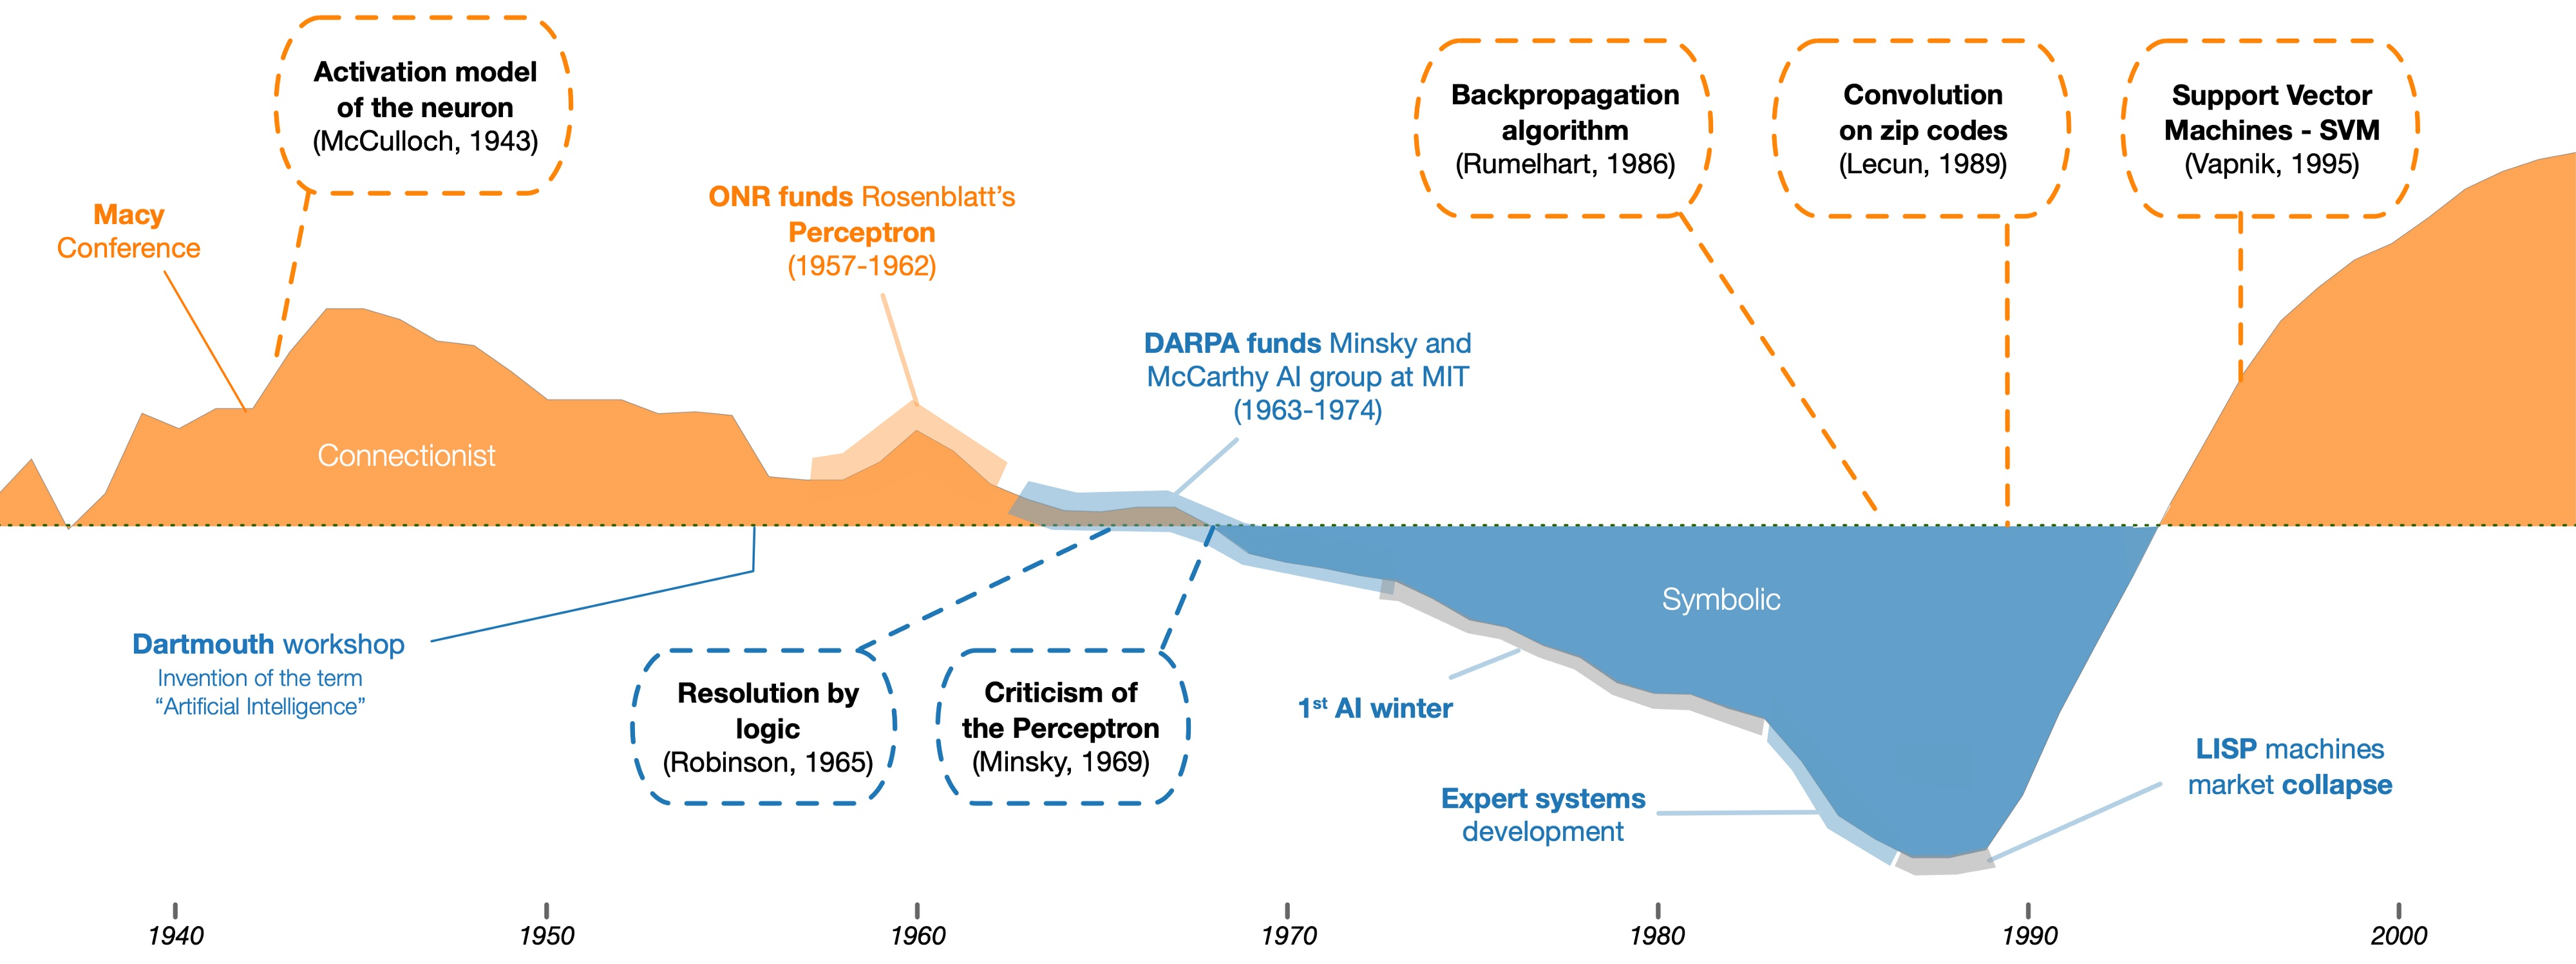
\includegraphics[width=\linewidth]{graphs/fig2.jpg}
        \caption*{60 лет истории исследований AI (по 2000 г.)}
    \end{figure}
\end{frame}

\begin{frame}{В чем сложность?}
    \begin{columns}
        \begin{column}{.43\linewidth}
            \begin{figure}
                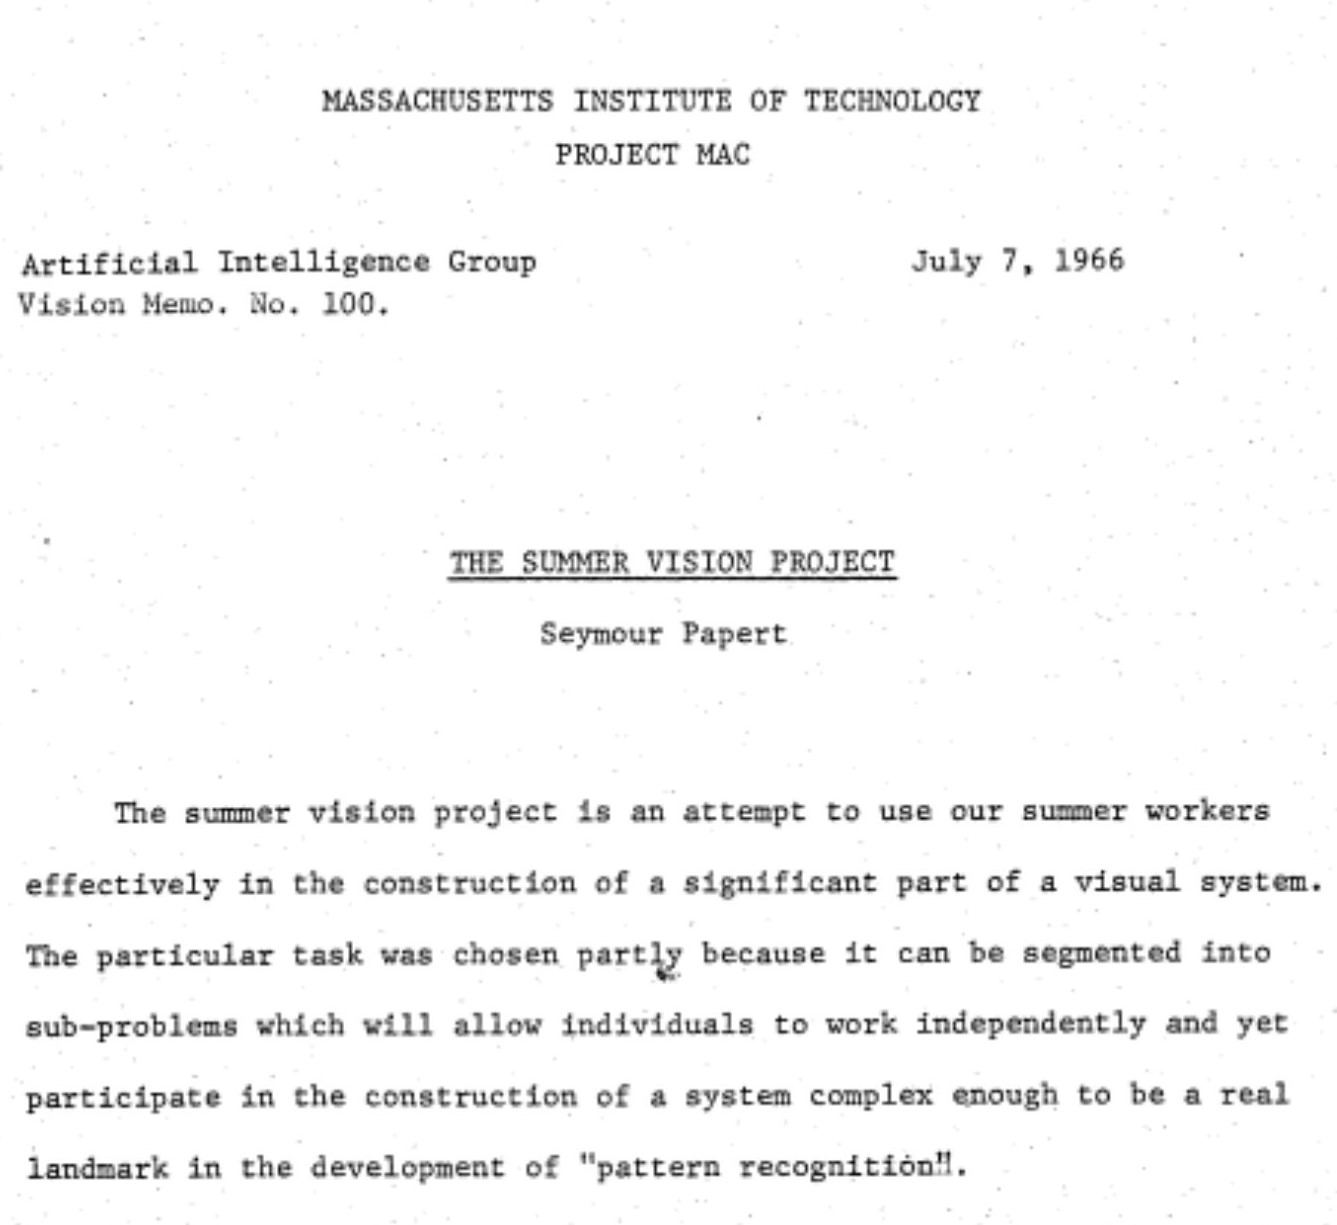
\includegraphics[width=\linewidth]{graphs/fig3_0.jpg}
                \caption*{Ожидание}
            \end{figure}
        \end{column}
        \pause{}
        \begin{column}{.24\linewidth}
            \begin{figure}
                
\includegraphics[width=\linewidth]{graphs/fig3_1.jpg}
                \caption*{Реальность}
            \end{figure}
        \end{column}
    \end{columns}
\end{frame}

\begin{frame}{В чем сложность?}
    \begin{columns}
        \begin{column}{.33\linewidth}
            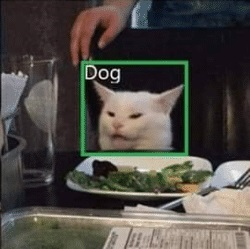
\includegraphics[width=\linewidth]{graphs/fig4_0.jpg}
        \end{column}
        \pause{}
        \begin{column}{.33\linewidth}
            
\includegraphics[width=\linewidth]{graphs/fig4_1.jpg}
        \end{column}
        \pause{}
        \begin{column}{.33\linewidth}
            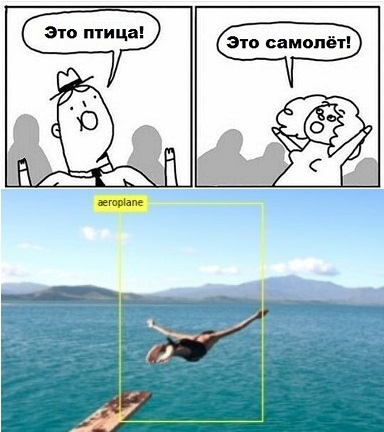
\includegraphics[width=\linewidth]{graphs/fig4_2.jpg}
        \end{column}
    \end{columns}
\end{frame}

\begin{frame}{Задача классификации изображений}
    Постановка задачи: для заданного изображения найти правильную метку из
    конечного дискретного набора
    \vfill
    \begin{columns}
        \begin{column}{.35\linewidth}
            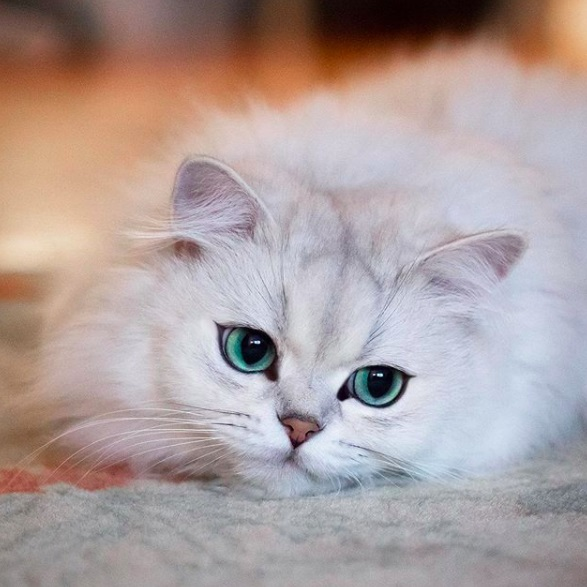
\includegraphics[width=\linewidth]{graphs/fig5.jpg}
        \end{column}
        \begin{column}{.65\linewidth}
            \( L = \{dog, cat, parrot, human, car, ninja, \ldots \} \) \\
            \hfill
            \vfill
            \( \Longrightarrow \quad \) cat
        \end{column}
    \end{columns}
\end{frame}

\begin{frame}{Задача классификации изображений}
    Более формально: построить функцию
    \( f(x) \rightarrow l, \quad l \in L \), \(x\) --- входное изображение
    \pause{}
    \vfill
    \begin{columns}
        \begin{column}{.49\linewidth}
            \begin{figure}
                \centering
                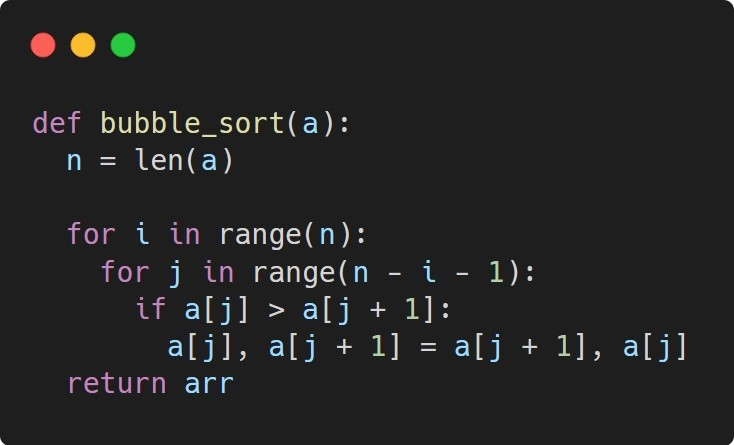
\includegraphics[width=\linewidth]{graphs/fig6_0.jpg}
                \caption*{Сортировка пузырьком}
            \end{figure}
        \end{column}
        \pause{}
        \begin{column}{.43\linewidth}
            \begin{figure}
                \centering
                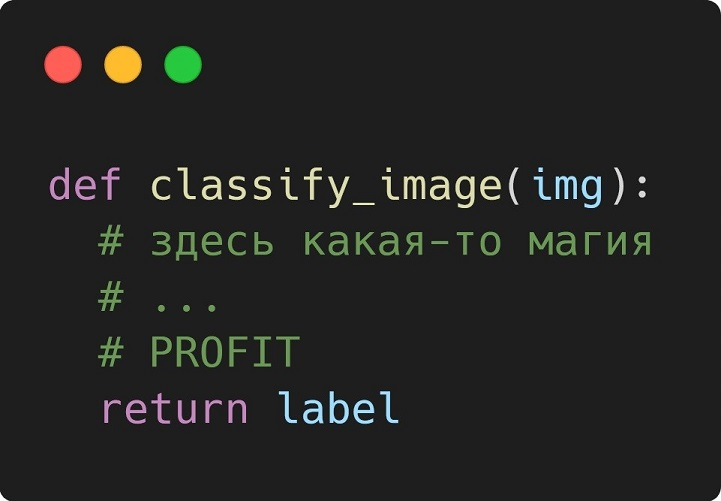
\includegraphics[width=\linewidth]{graphs/fig6_1.jpg}
                \caption*{Классификация}
            \end{figure}
        \end{column}
    \end{columns}
\end{frame}

\begin{frame}{Семантический разрыв (semantic gap)}
    \begin{columns}
        \begin{column}{.35\linewidth}
            \begin{figure}
                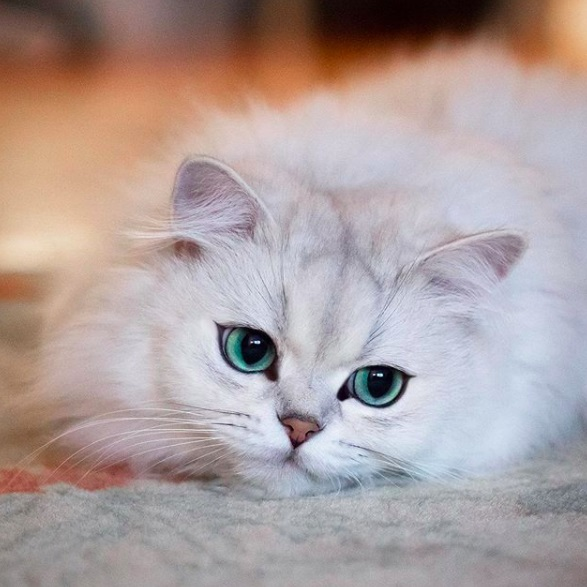
\includegraphics[width=\linewidth]{graphs/fig5.jpg}
                \caption*{Что видим мы: кошка}
            \end{figure}
            
        \end{column}
        \pause{}
        \begin{column}{.65\linewidth}
            \begin{figure}
                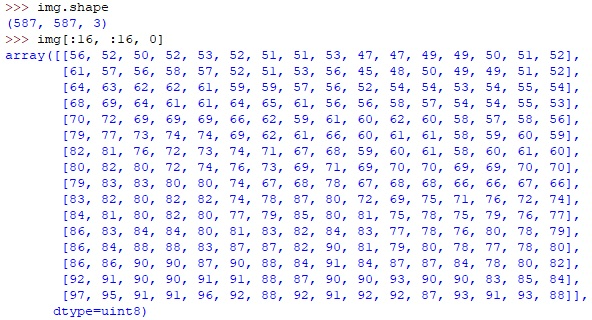
\includegraphics[width=\linewidth]{graphs/fig7.jpg}
                \caption*{Что видит компьютер: WTF}
            \end{figure}
        \end{column}
    \end{columns}
\end{frame}

\begin{frame}{Сложности: смена ракурса}
    \begin{figure}
        \begin{subfigure}[b]{.325\linewidth}
            \centering
            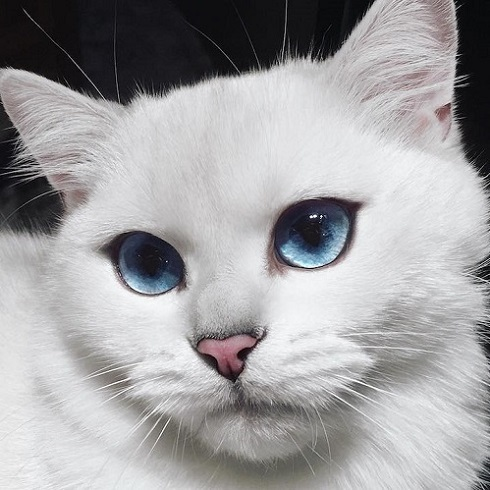
\includegraphics[width=\linewidth]{graphs/fig8_0.jpg}
        \end{subfigure}
        \begin{subfigure}[b]{.325\linewidth}
            \centering
            
\includegraphics[width=\linewidth]{graphs/fig8_1.jpg}
        \end{subfigure}
        \begin{subfigure}[b]{.325\linewidth}
            \centering
            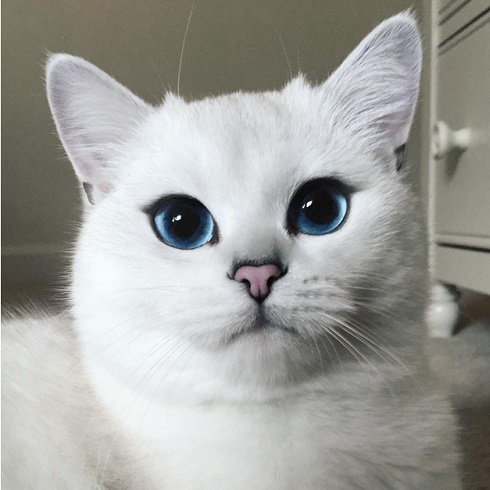
\includegraphics[width=\linewidth]{graphs/fig8_2.jpg}
        \end{subfigure}
    \end{figure}
\end{frame}

\begin{frame}{Сложности: разное освещение}
    \begin{figure}
        \begin{subfigure}[b]{.3\linewidth}
            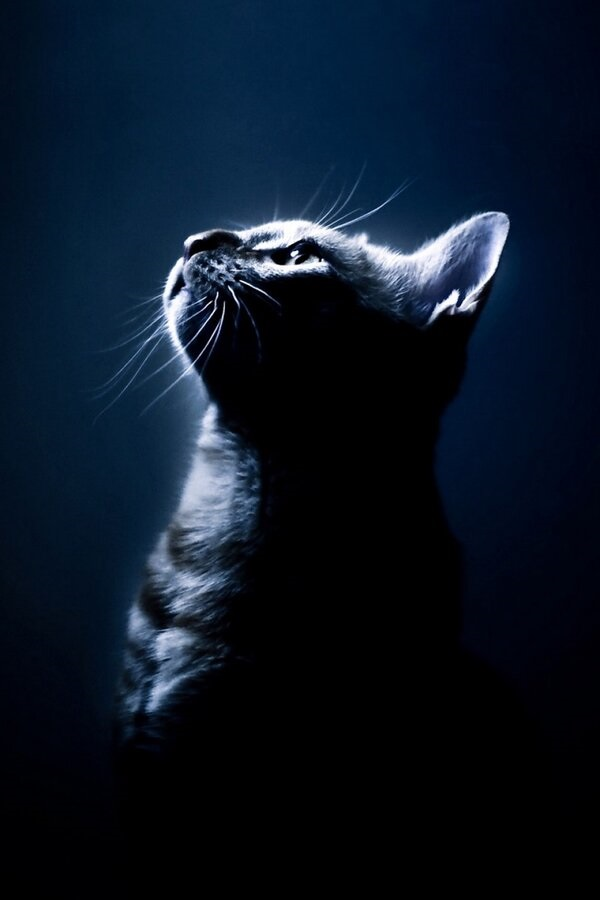
\includegraphics[width=\linewidth]{graphs/fig9_0.jpg}
        \end{subfigure}
        \begin{subfigure}[b]{.3\linewidth}
            
\includegraphics[width=\linewidth]{graphs/fig9_1.jpg}
        \end{subfigure}
        \begin{subfigure}[b]{.3\linewidth}
            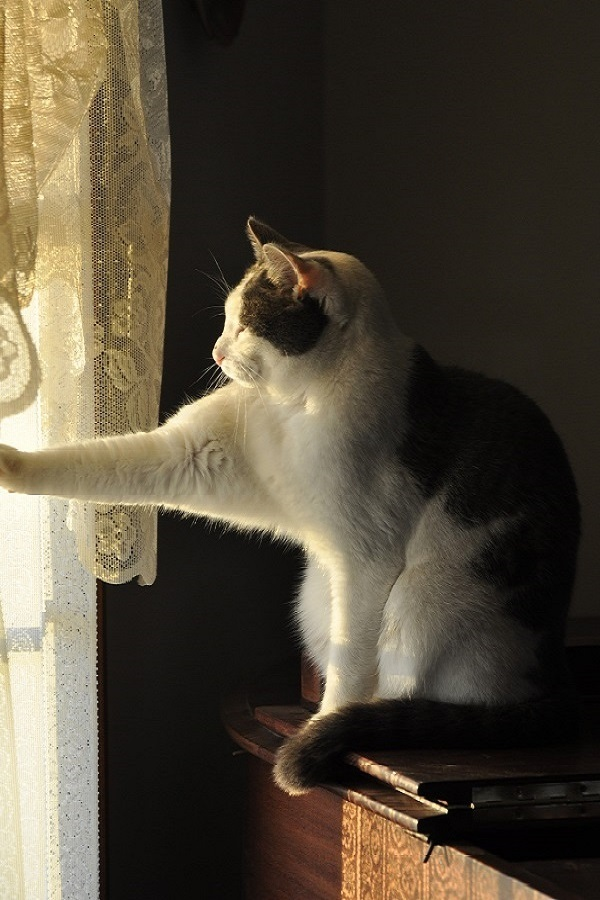
\includegraphics[width=\linewidth]{graphs/fig9_2.jpg}
        \end{subfigure}
    \end{figure}
\end{frame}

\begin{frame}{Сложности: вариация форм (cats are liquid)}
    \begin{figure}
        \begin{subfigure}[b]{.3\linewidth}
            
\includegraphics[width=\linewidth]{graphs/fig10_0.jpg}
        \end{subfigure}
        \begin{subfigure}[b]{.3\linewidth}
            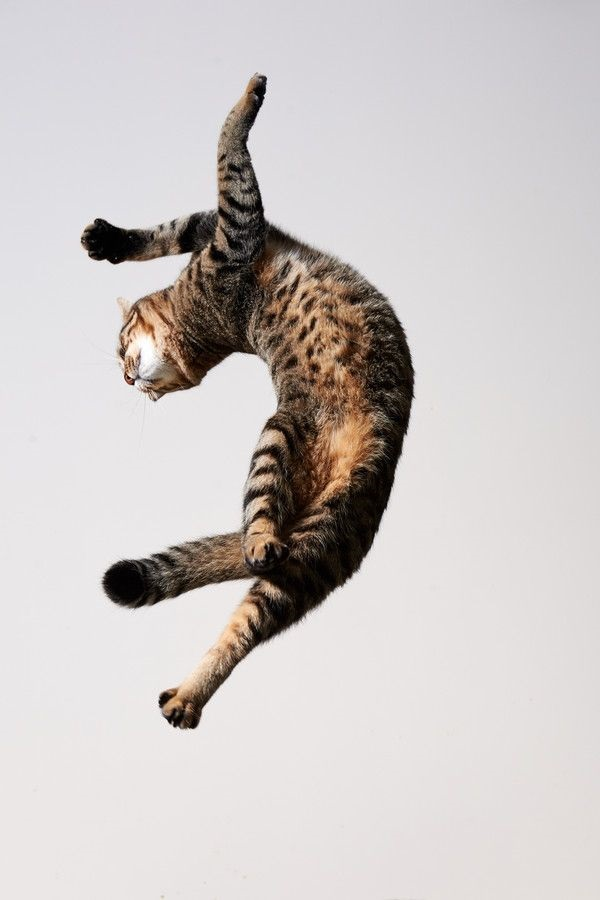
\includegraphics[width=\linewidth]{graphs/fig10_1.jpg}
        \end{subfigure}
        \begin{subfigure}[b]{.3\linewidth}
            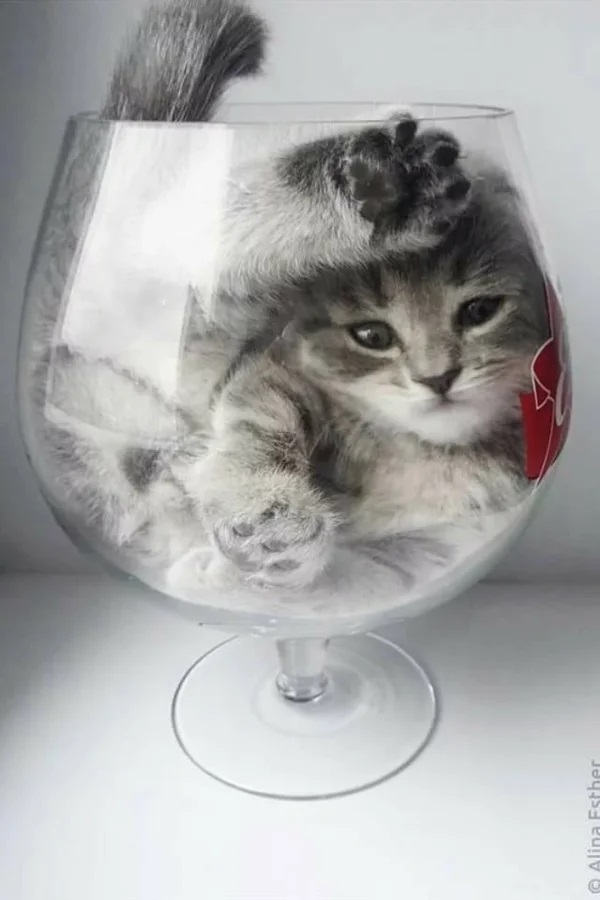
\includegraphics[width=\linewidth]{graphs/fig10_2.jpg}
        \end{subfigure}
    \end{figure}
\end{frame}

\begin{frame}{Сложности: внутриклассовая вариативность}
    \centering
    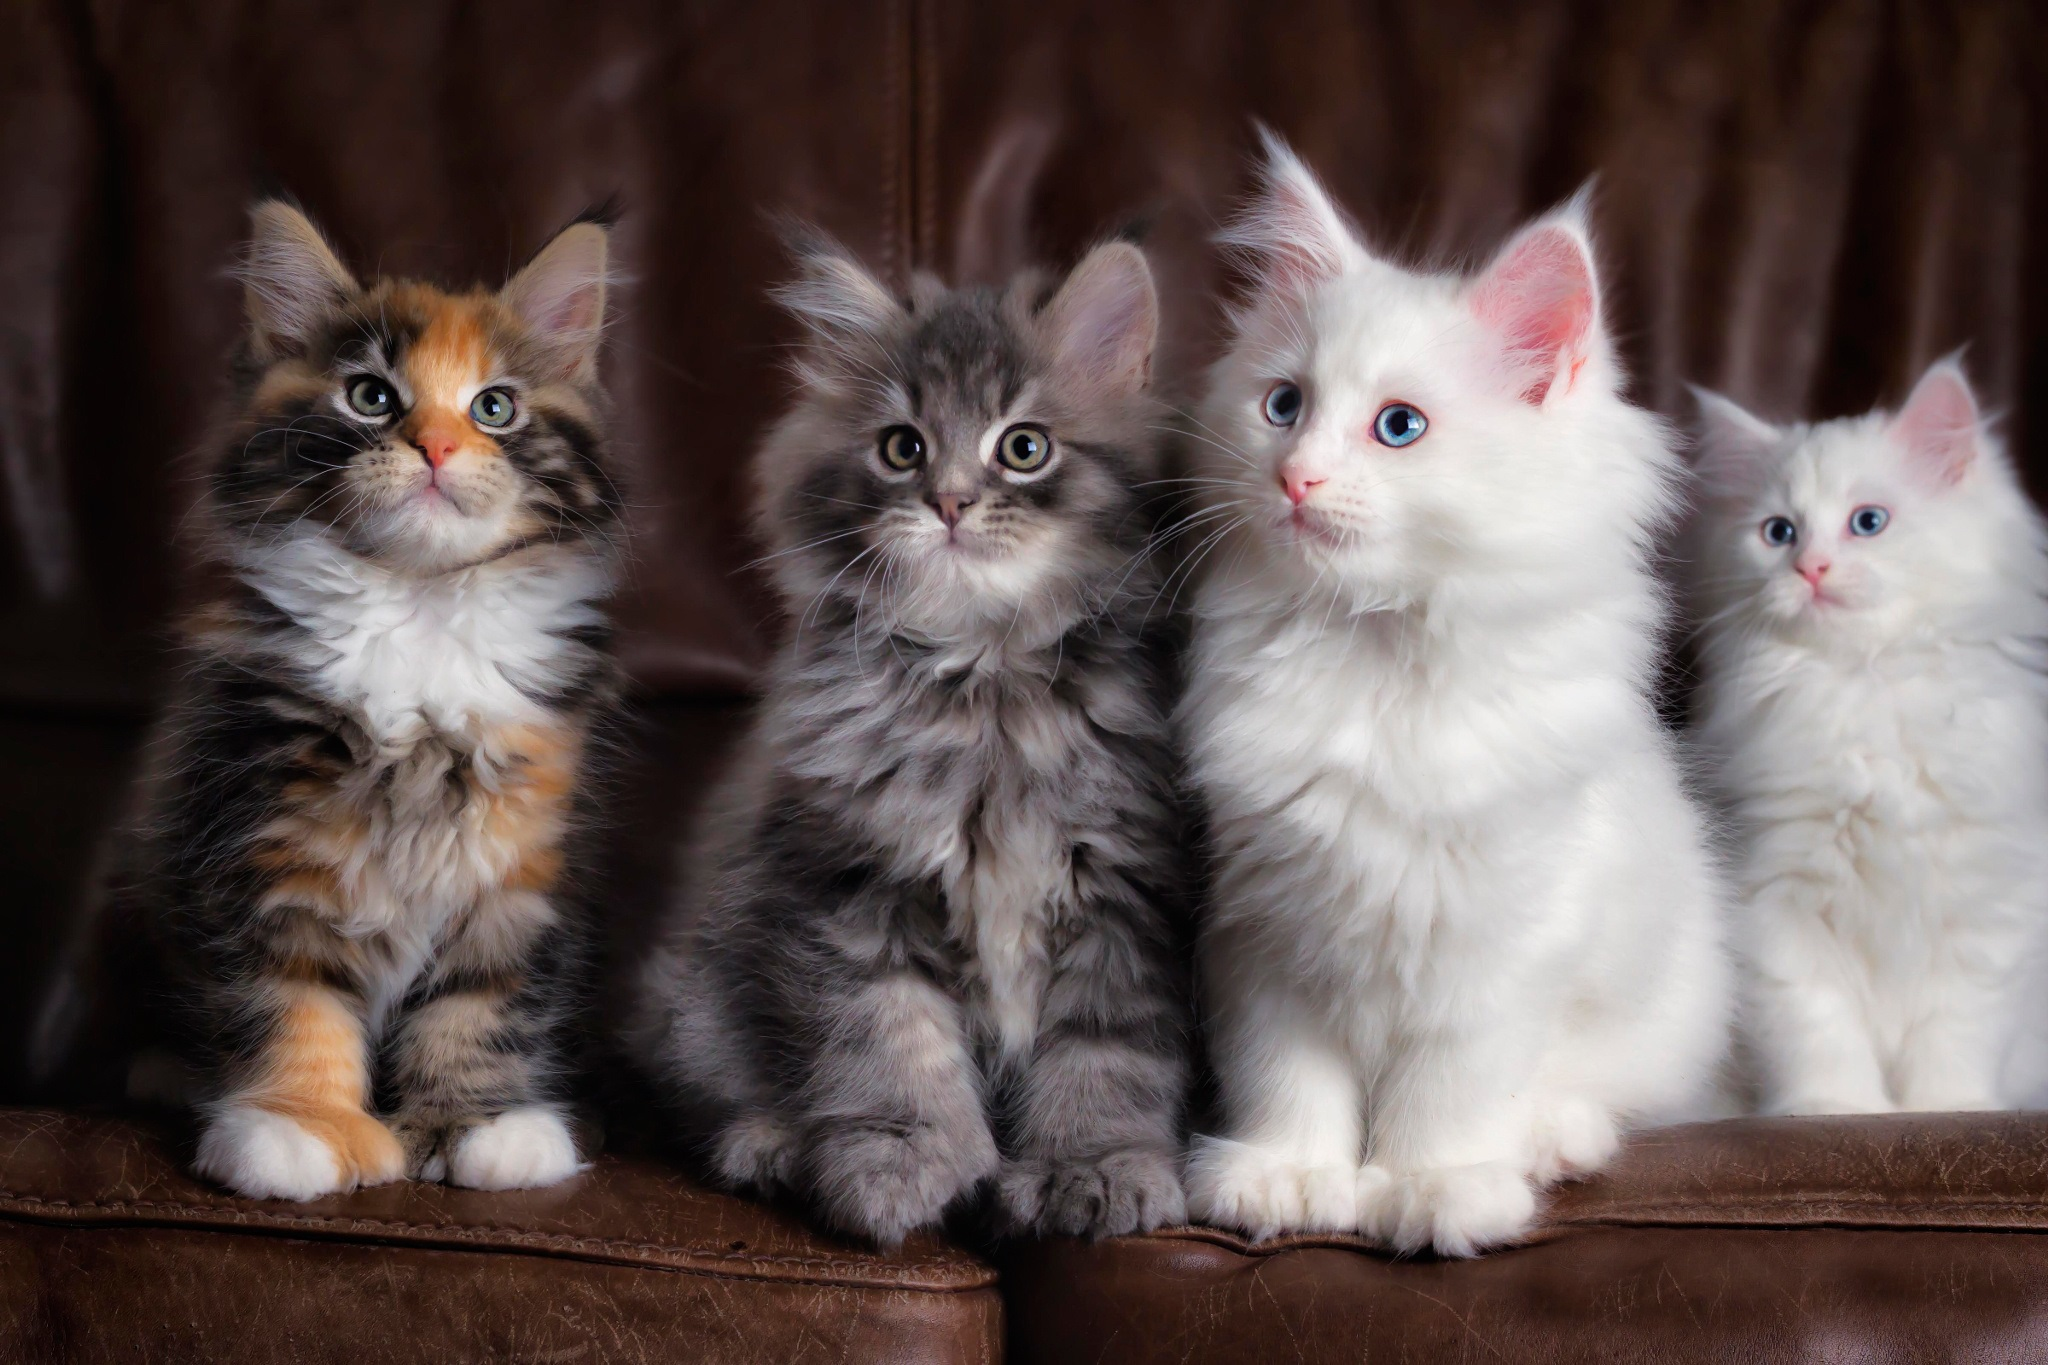
\includegraphics[width=.71\linewidth]{graphs/fig11.jpg}
\end{frame}

\begin{frame}{Задача классификации изображений}
    \centering
    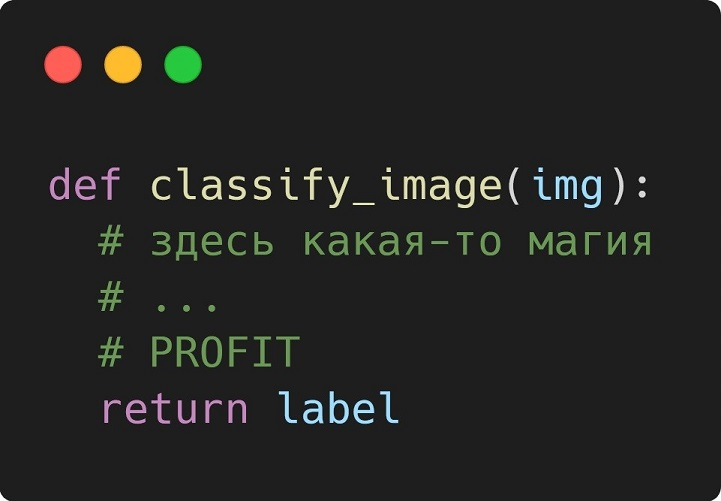
\includegraphics[width=.5\linewidth]{graphs/fig6_1.jpg}

    \textbf{Очевидным} способом построить такую функцию так и не получилось
\end{frame}

\begin{frame}{Задача классификации изображений}
    Конечно, было предпринято множество попыток, например
    \vfill
    \begin{columns}
        \begin{column}{.25\linewidth}
            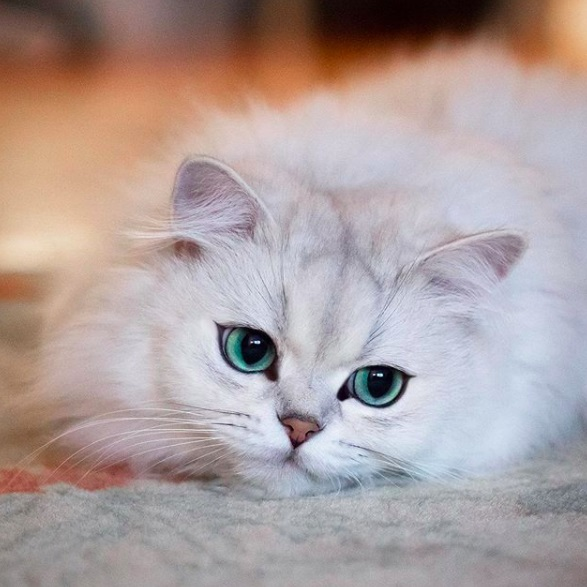
\includegraphics[width=\linewidth]{graphs/fig5.jpg}
        \end{column}
        \pause{}
        \begin{column}{.15\linewidth}
            \centering
            \( \longrightarrow \) \\
            границы
        \end{column}
        \begin{column}{.25\linewidth}
            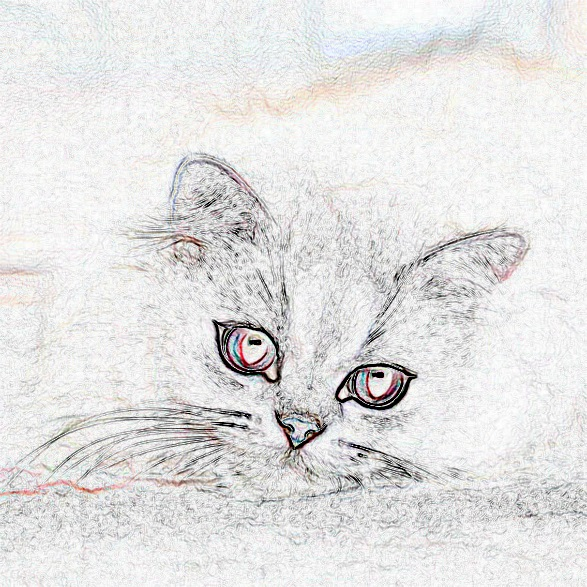
\includegraphics[width=\linewidth]{graphs/fig12_1.jpg}
        \end{column}
        \pause{}
        \begin{column}{.15\linewidth}
            \centering
            \( \longrightarrow \) \\
            углы
        \end{column}
        \begin{column}{.07\linewidth}
            
\includegraphics[width=\linewidth]{graphs/fig12_2.jpg}
        \end{column}
        \pause{}
        \begin{column}{.13\linewidth}
            \centering
            \( \longrightarrow  \) \\
            \( ? \)
        \end{column}
    \end{columns}
\end{frame}

\begin{frame}{A wild machine learning appears}
    \centering
    
\includegraphics[width=.715\linewidth]{graphs/fig13.jpg}
\end{frame}

\begin{frame}{Машинное обучение: подход от данных}
    \begin{itemize}
        \item Алгоритмы \textbf{машинного обучения} (machine learning, ML) ---
        класс алгоритмов, которые \textbf{не программируются явно}, но
        \textbf{подстраиваются под предоставленные данные (обучающую выборку)}
        \pause{}
        \item \textbf{Обучающая выборка} --- набор примеров с правильными
        ответами
    \end{itemize}
    \begin{figure}
        \begin{subfigure}[b]{.1\linewidth}
            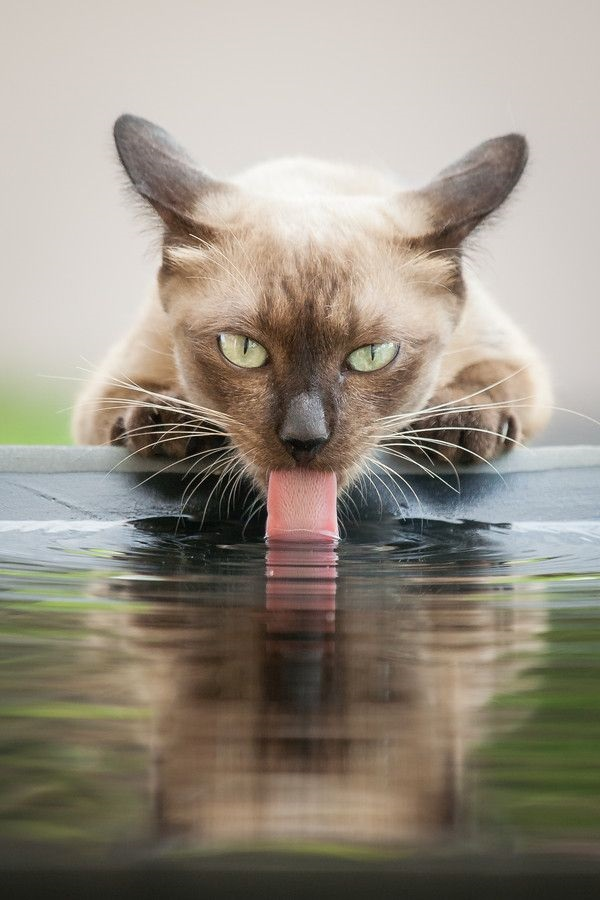
\includegraphics[width=\linewidth]{graphs/fig14_0.jpg}
            \subcaption*{`cat'}
        \end{subfigure}
        \begin{subfigure}[b]{.1\linewidth}
            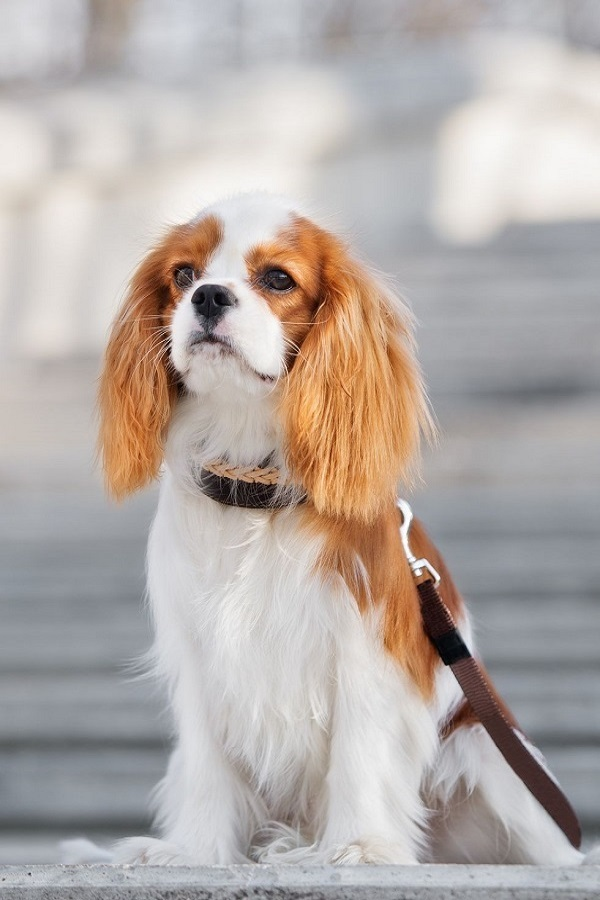
\includegraphics[width=\linewidth]{graphs/fig14_1.jpg}
            \subcaption*{`dog'}
        \end{subfigure}
        \begin{subfigure}[b]{.1\linewidth}
            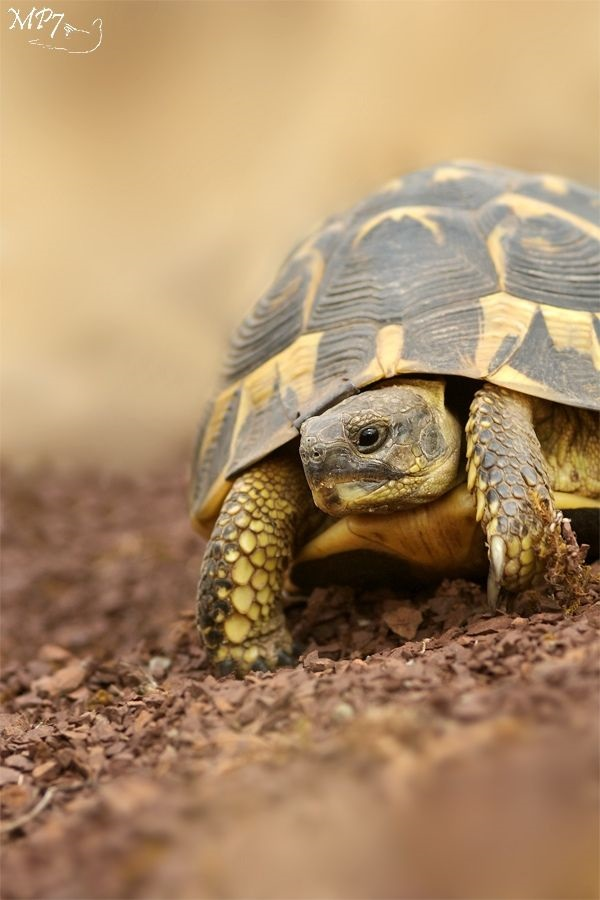
\includegraphics[width=\linewidth]{graphs/fig14_2.jpg}
            \subcaption*{`ninja'}
        \end{subfigure}
        \begin{subfigure}[b]{.1\linewidth}
            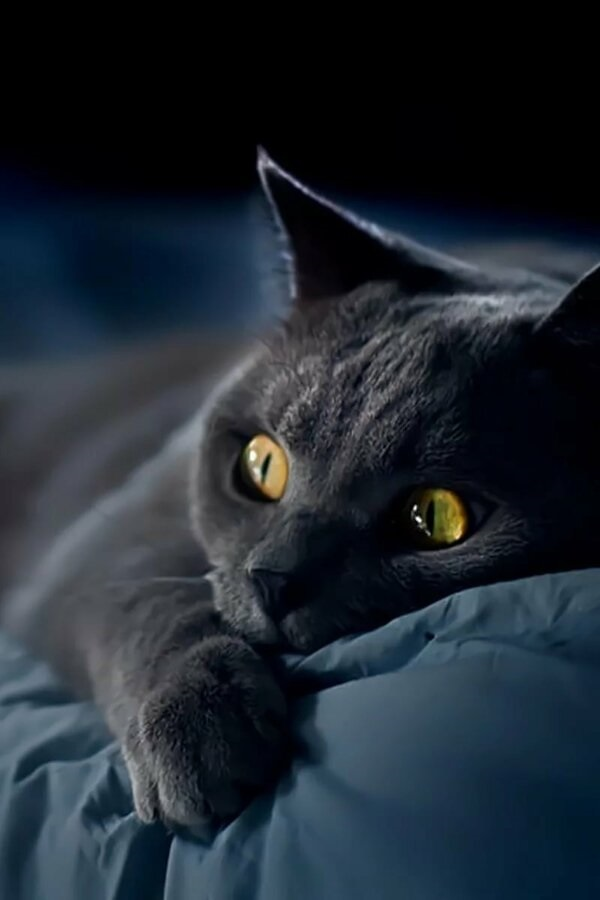
\includegraphics[width=\linewidth]{graphs/fig14_3.jpg}
            \subcaption*{`cat'}
        \end{subfigure}
        \begin{subfigure}[b]{.1\linewidth}
            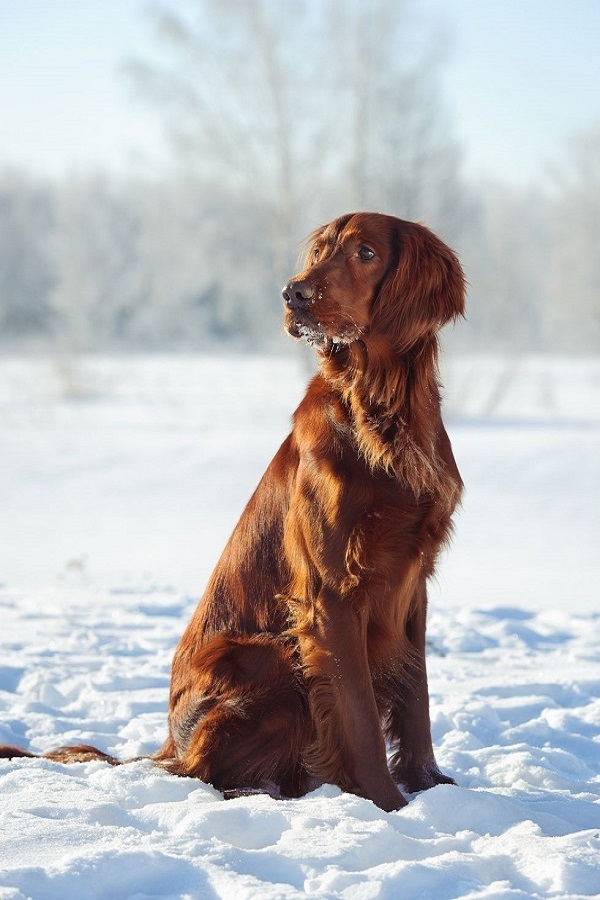
\includegraphics[width=\linewidth]{graphs/fig14_4.jpg}
            \subcaption*{`dog'}
        \end{subfigure}
        \begin{subfigure}[b]{.1\linewidth}
            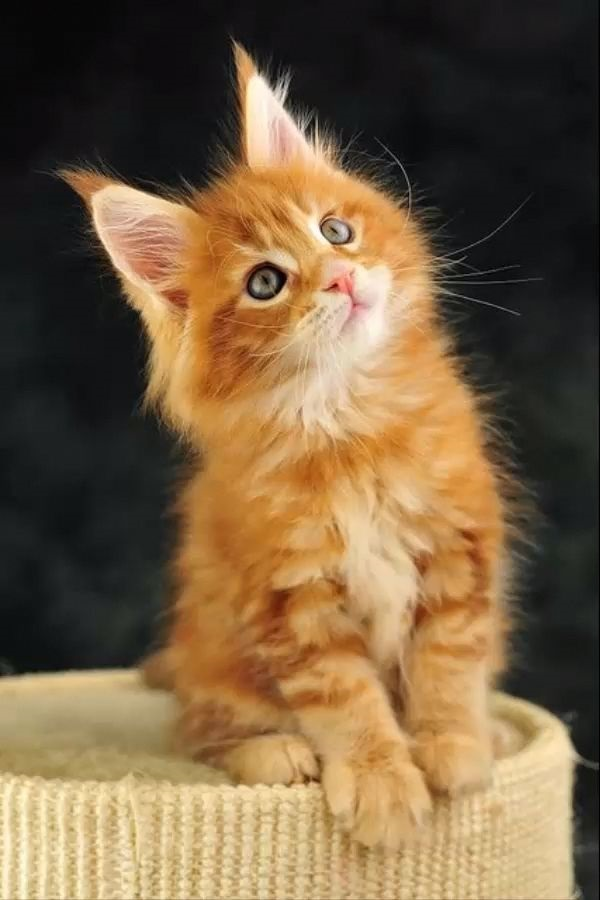
\includegraphics[width=\linewidth]{graphs/fig14_5.jpg}
            \subcaption*{`cat'}
        \end{subfigure}
        \begin{subfigure}[b]{.1\linewidth}
            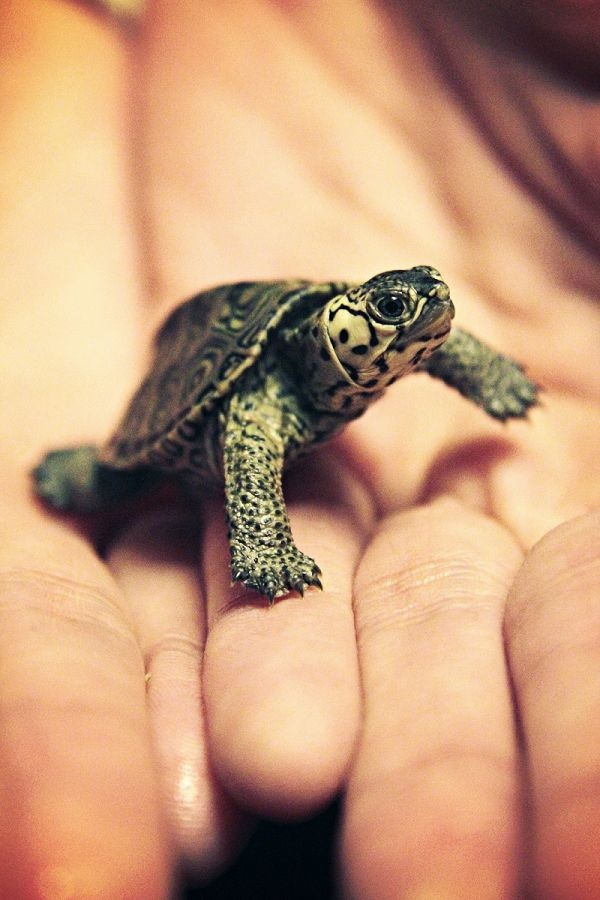
\includegraphics[width=\linewidth]{graphs/fig14_6.jpg}
            \subcaption*{`ninja'}
        \end{subfigure}
        \begin{subfigure}[b]{.1\linewidth}
            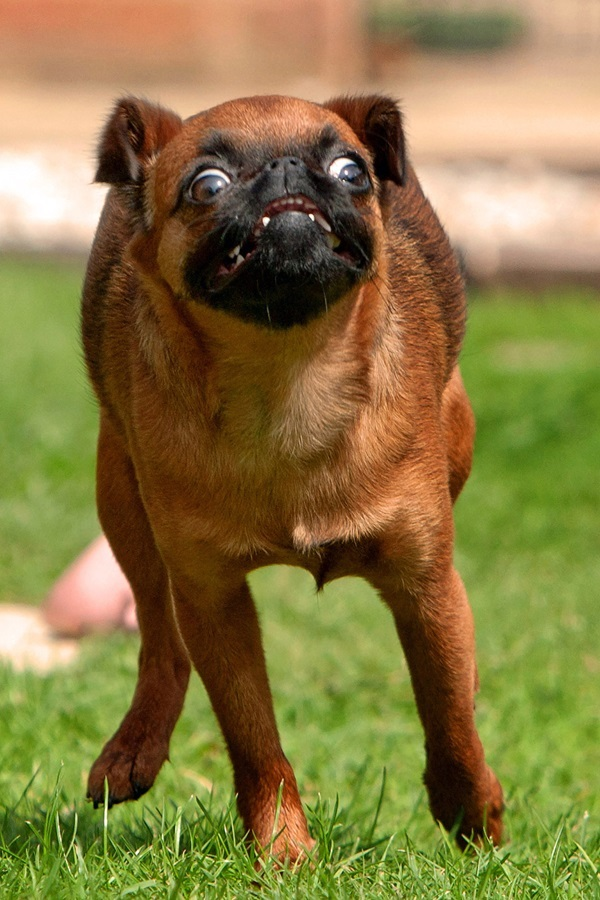
\includegraphics[width=\linewidth]{graphs/fig14_7.jpg}
            \subcaption*{`dog'}
        \end{subfigure}
        \begin{subfigure}[b]{.1\linewidth}
            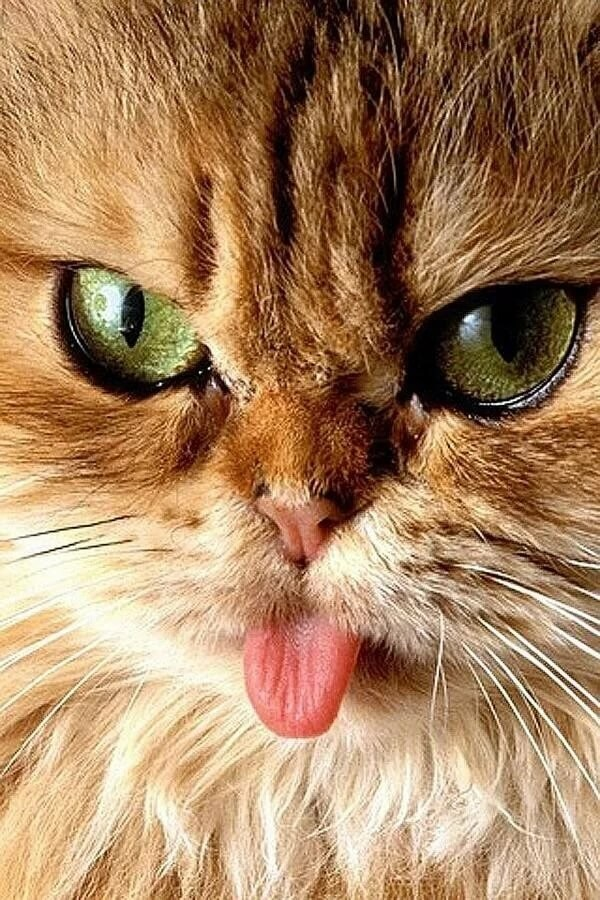
\includegraphics[width=\linewidth]{graphs/fig14_8.jpg}
            \subcaption*{`cat'}
        \end{subfigure}
        \caption*{Так может выглядеть обучающая выборка}
    \end{figure}
\end{frame}

\begin{frame}{Машинное обучение: подход от данных}
    \begin{columns}[T]
        \begin{column}{.4\linewidth}
            \begin{figure}
                \caption*{Таким образом, наша функция}
                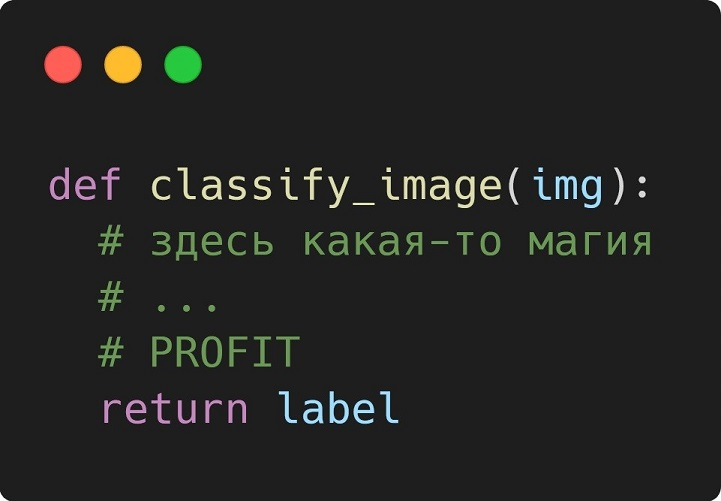
\includegraphics[width=\linewidth]{graphs/fig6_1.jpg}
            \end{figure}
        \end{column}
        \pause{}
        \begin{column}{.6\linewidth}
            \begin{figure}
                \caption*{превращается в две:}
                \begin{subfigure}[t]{.57\linewidth}
                    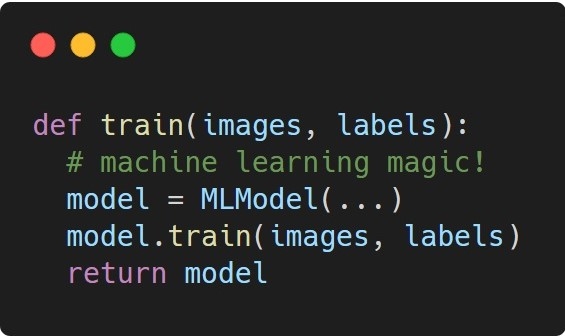
\includegraphics[width=\linewidth]{graphs/fig15_0.jpg}
                \end{subfigure}
                \begin{subfigure}[b]{.57\linewidth}
                    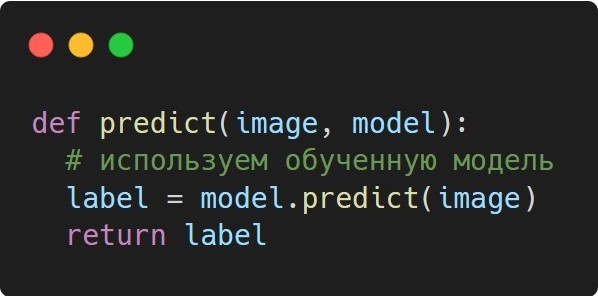
\includegraphics[width=\linewidth]{graphs/fig15_1.jpg}
                \end{subfigure}
            \end{figure}
        \end{column}
    \end{columns}
\end{frame}

\begin{frame}{Разница подходов}
    \begin{columns}[T]
        \begin{column}{.44\linewidth}
            \begin{figure}
                \caption*{Software Engineering}
                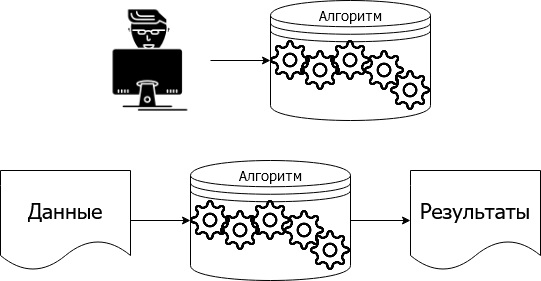
\includegraphics[width=\linewidth]{graphs/fig16_0.jpg}
            \end{figure}
        \end{column}
        \pause{}
        \begin{column}{.54\linewidth}
            \begin{figure}
                \caption*{Machine Learning}
                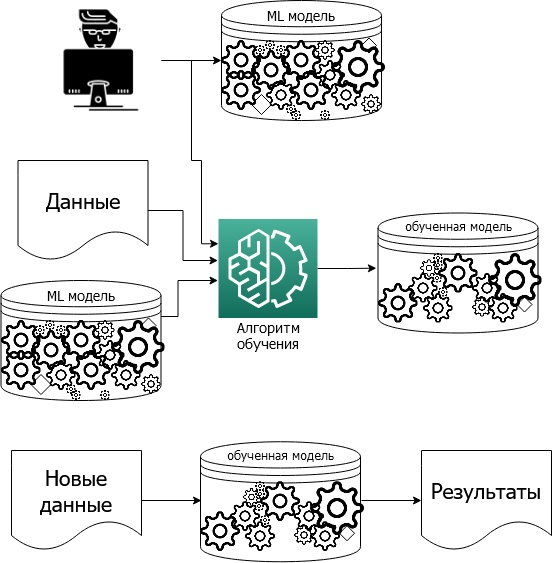
\includegraphics[width=.68\linewidth]{graphs/fig16_1.jpg}
            \end{figure}
        \end{column}
    \end{columns}
\end{frame}

\begin{frame}{Машинное обучение: подход от данных}
    Смысл от применения машинного обучения появляется, когда:
    \begin{itemize}
        \item мы не можем создать точный алгоритм решения задачи, потому что
        слишком мало понимаем лежащие в её основах процессы и
        \textbf{не можем построить} точную модель этих процессов (в отличии,
        скажем, от моделей в физике)
        \pause{}
        \item или модель есть, но ее полный расчет невозможен ввиду вычислительных
        ограничений (как в квантовой химии) 
        \pause{}
        \item но при этом мы можем собрать \textbf{большое} количество данных с примерами
        правильного решения задачи (обучающую выборку)
    \end{itemize}
\end{frame}

\begin{frame}{Минутка философии}
    Осмыслим специфику подобного подхода:
    \begin{itemize}
        \item Методы машинного обучения пытаются \textbf{восстанавливать модели} на
        основе \textbf{данных}, а не исходя из понимания природы
        \pause{}
        \item ``Золотое'' правило машинного обучения
    \end{itemize}
    \begin{figure}
        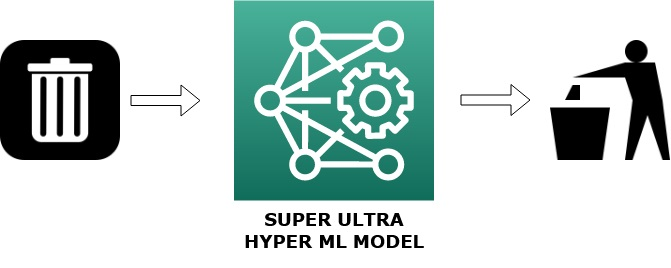
\includegraphics[width=.49\linewidth]{graphs/fig17.jpg}
        \caption*{garbade in --- garbage out}
    \end{figure}
\end{frame}

\begin{frame}{Минутка философии}
    \begin{itemize}
        \item Машинное обучение находится на стыке матстатистики, программирования и
        вычислительной математики (численной оптимизации)
        \pause{}
        \item ML алгоритмы являются статистическими по своей сути, поэтому при их
        использовании необходимо допущение об ``устойчивости'' процесса
        \pause{}
        \item Суть и основная проблема машинного обучения: модель учится на некоторой
        конечной выборке данных, а мы хотим чтобы она работала в будущем, на
        новых данных
        \pause{}
        \item Из-за этого возникают специфичные проблемы: недообучение,
        переобучение, протечки
        \pause{}
        \item А также используются специфичные способы проверки работоспособности модели
    \end{itemize}
\end{frame}

\begin{frame}{Если же это не учитывать, то\ldots}
    \begin{figure}
        \caption*{\ldots результат выйдет примерно таким}
        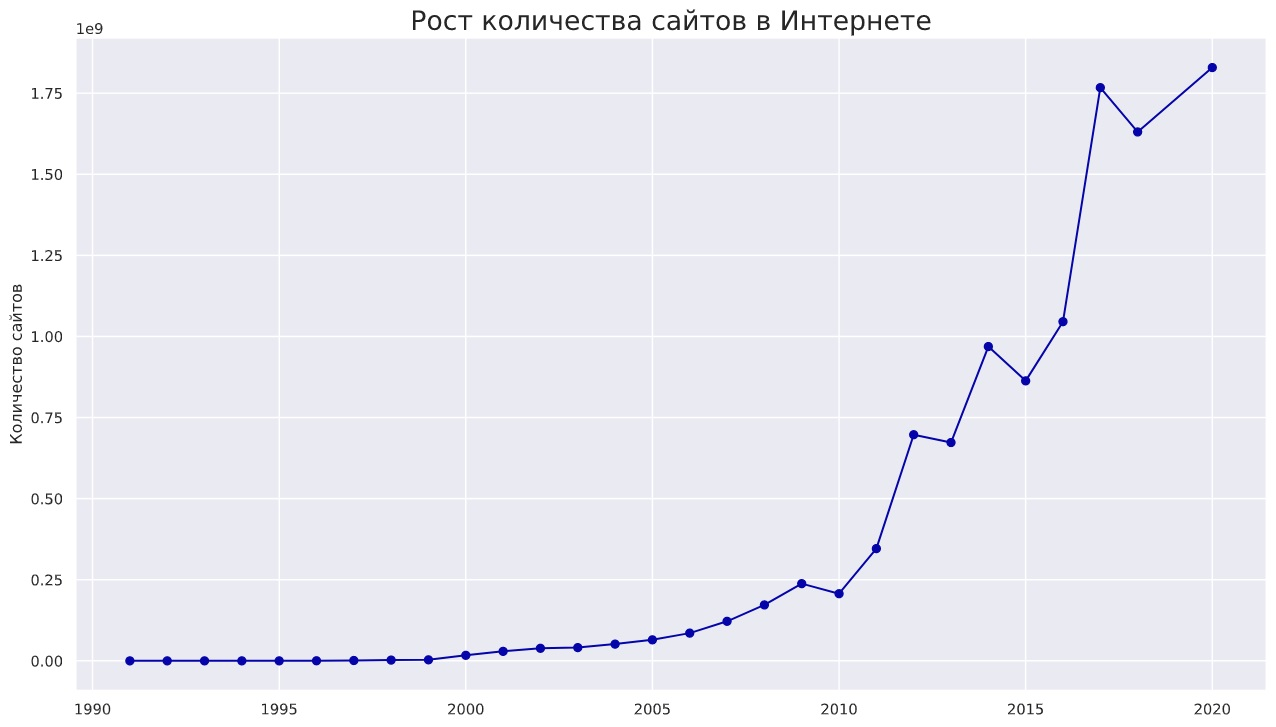
\includegraphics[width=.3\linewidth]{graphs/fig18.jpg}
    \end{figure}
\end{frame}

\begin{frame}{Вернемся к истории}
    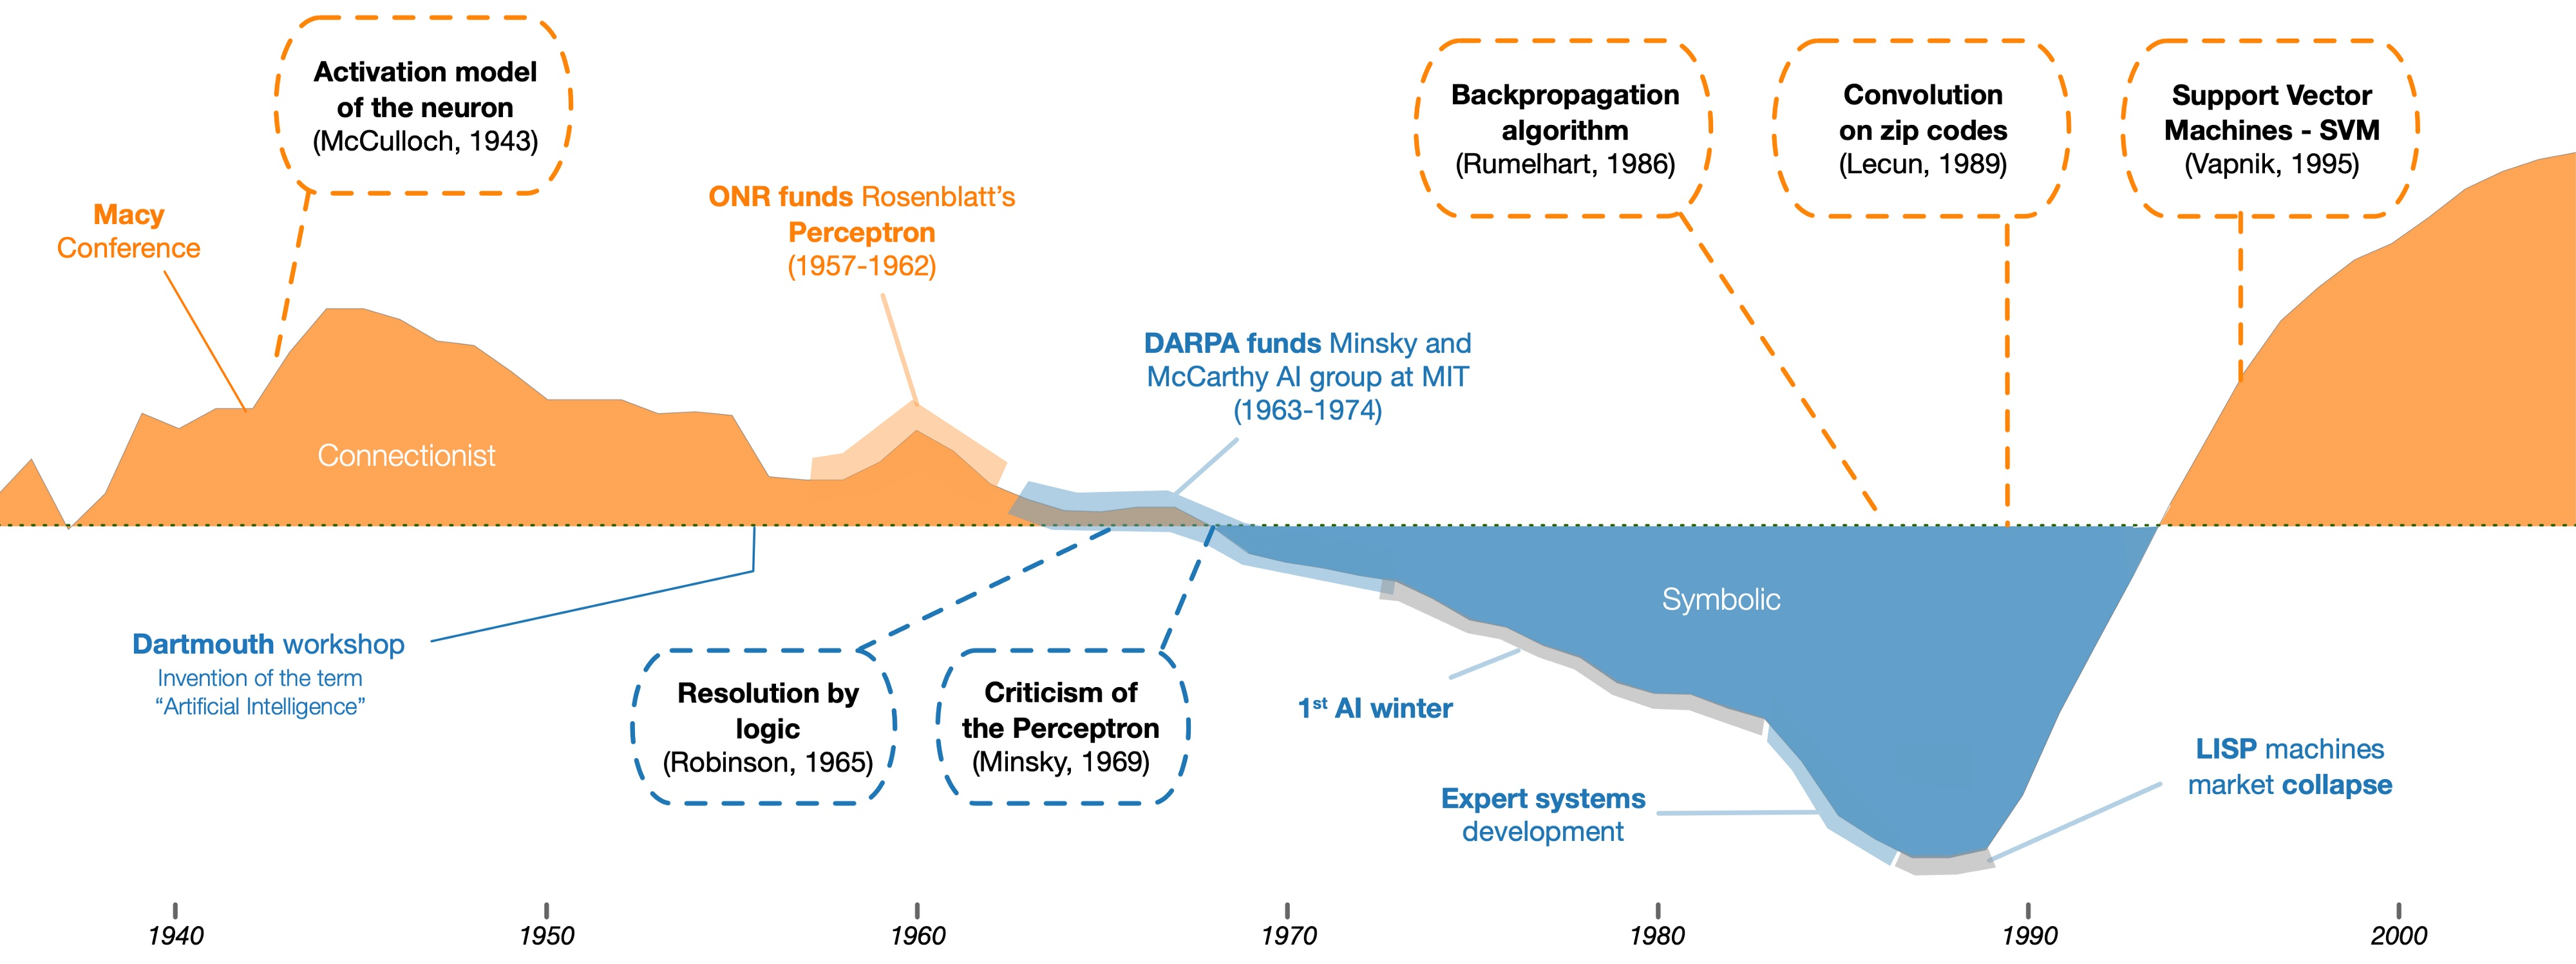
\includegraphics[width=\linewidth]{graphs/fig2.jpg}
\end{frame}

\begin{frame}{Вернемся к истории}
    \large
    \begin{itemize}
        \item Искусственные нейросети были изобретены не несколько лет назад,
        первые модели появились ещё в довоенное время
        \pause{}
        \item Со времени своего изобретения они прошли несколько пиков популярности
        и забвения
        \pause{}
        \item Современный период популярности нейронных сетей начался в 2012 году
        \item Почему именно сейчас успех всё-таки настиг нейросети?
    \end{itemize}
\end{frame}

\begin{frame}{Первая половина успеха: данные}
    \centering
    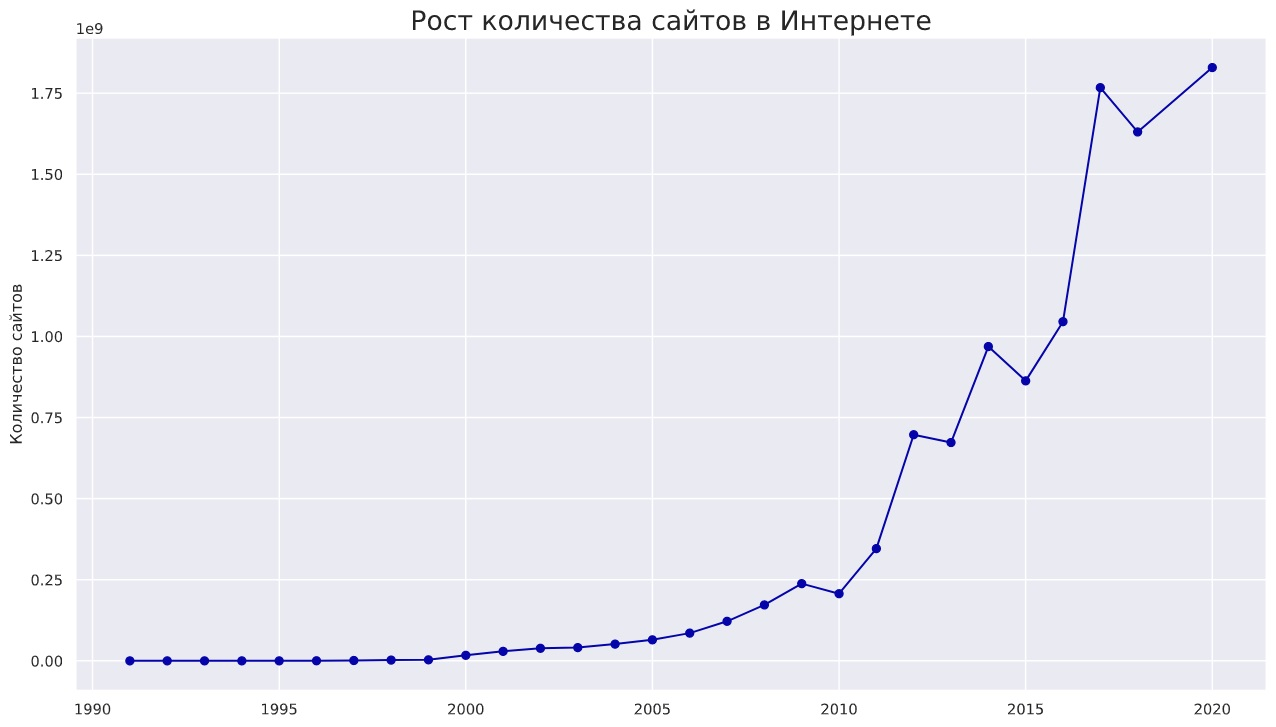
\includegraphics[width=.84\linewidth]{graphs/fig19.jpg}
\end{frame}

\begin{frame}{Первая половина успеха: данные}
    \centering
    
\includegraphics[width=\linewidth]{graphs/fig20.jpg}
\end{frame}

\begin{frame}{Первая половина успеха: данные}
    \centering
    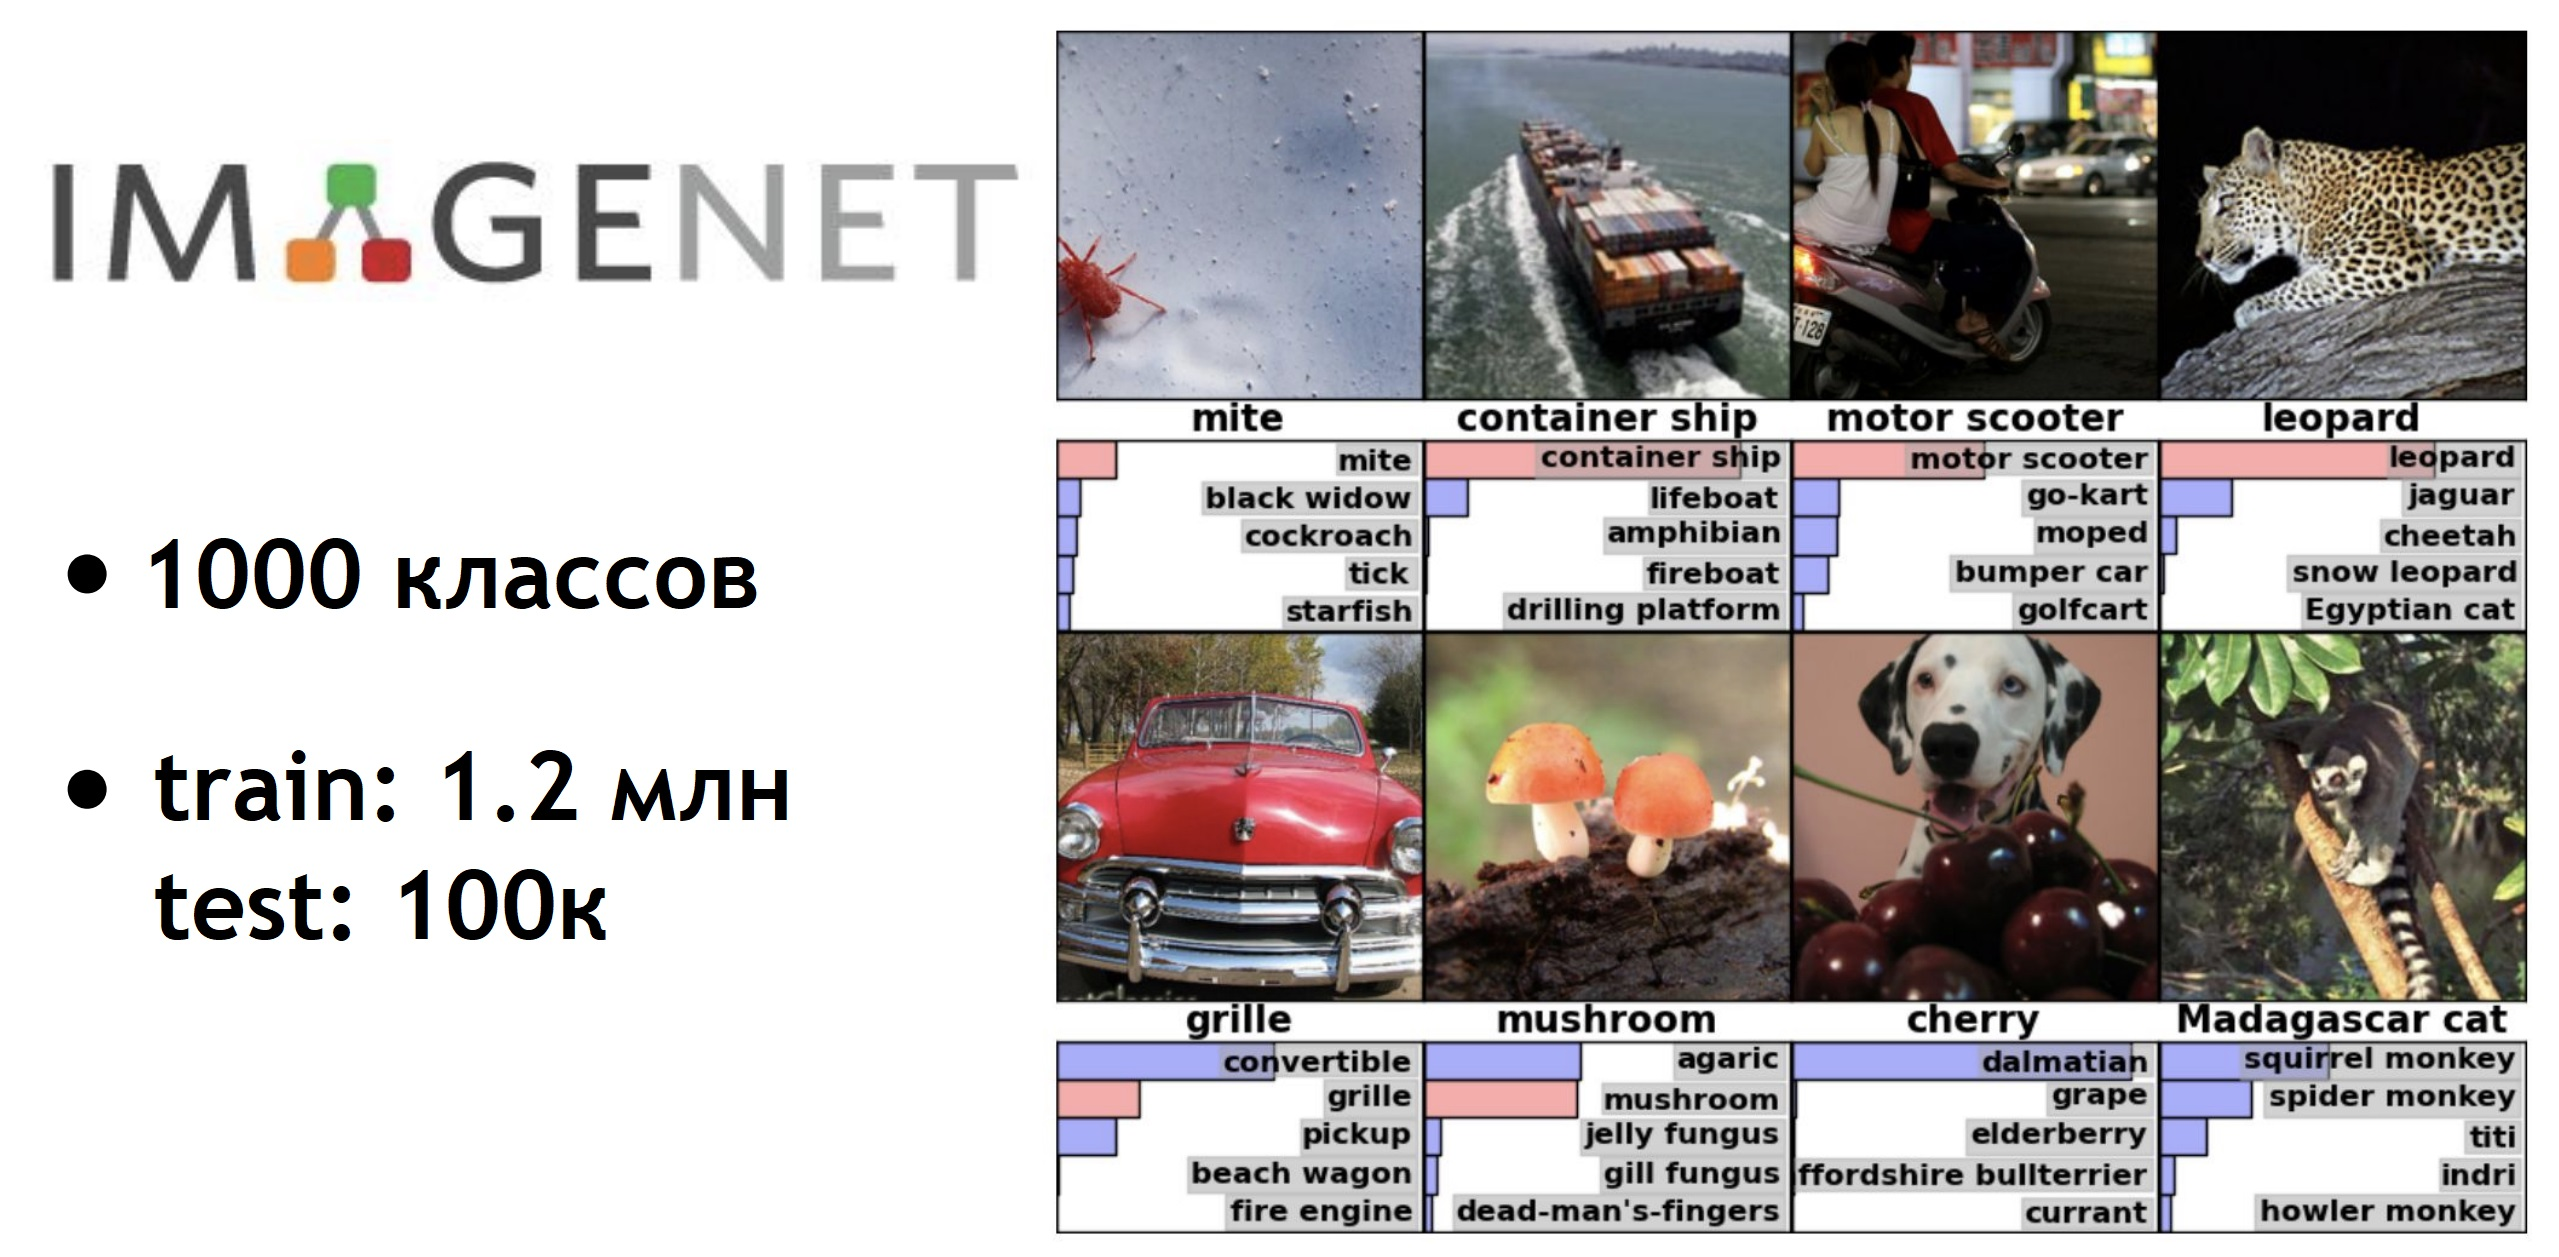
\includegraphics[width=.97\linewidth]{graphs/fig21.jpg}
\end{frame}

\begin{frame}{Первая половина успеха: данные}
    \begin{itemize}
        \item C 2010 года проводится ILSVRC --- ImageNet Large Scale Visual
        Recognition Competition
        \item Это соревнование, помимо открытого доступа к большому датасету
        ImageNet, дало научному сообществу простой способ сравнивать
        различные модели, что сильно ускорило прогресс в области
    \end{itemize}
\end{frame}

\begin{frame}{Однако, одних только данных недостаточно\ldots}
    \begin{figure}
        \begin{subfigure}{.49\linewidth}
            \centering
            
\includegraphics[width=.76\linewidth]{graphs/fig22_0.jpg}
            \caption*{60е: нет эффективных алгоритмов}
        \end{subfigure}
        \pause{}
        \begin{subfigure}{.49\linewidth}
            \centering
            \includegraphics[width=.57\linewidth]{graphs/fig22_1.jpg}
            \caption*{90е: нет вычислительных мощностей}
        \end{subfigure}
    \end{figure}
\end{frame}

\begin{frame}{Вторая половина успеха: компьютерные игры}
    \centering
    \includegraphics[width=.83\linewidth]{graphs/fig23.jpg}
\end{frame}

\begin{frame}{Вторая половина успеха: вычисления}
    \centering
    \includegraphics[width=.74\linewidth]{graphs/fig24.jpg}
\end{frame}

\begin{frame}{Вторая половина успеха: вычисления}
    \begin{columns}
        \begin{column}{.5\linewidth}
            \centering
            \includegraphics[width=\linewidth]{graphs/fig25_0.jpg}
        \end{column}
        \begin{column}{.5\linewidth}
            \centering
            \includegraphics[width=\linewidth]{graphs/fig25_1.jpg}
        \end{column}
    \end{columns}
\end{frame}

\begin{frame}{Вторая половина успеха: вычисления}
    \centering
    \includegraphics[width=.91\linewidth]{graphs/fig26.jpg}
\end{frame}

\begin{frame}{Вторая половина успеха: вычисления}
    \centering
    \includegraphics[width=.86\linewidth]{graphs/fig27.jpg}
\end{frame}

\begin{frame}{Ренессанс глубокого обучения}
    \centering
    \includegraphics[width=.75\linewidth]{graphs/fig28.jpg}
\end{frame}

\begin{frame}{Ренессанс глубокого обучения}
    \centering
    \includegraphics[width=.85\linewidth]{graphs/fig29.jpg}
\end{frame}

\begin{frame}{Ренессанс глубокого обучения}
    \centering
    \includegraphics[width=.63\linewidth]{graphs/fig30.jpg}
\end{frame}

\begin{frame}{Задачи машинного обучения}
    \centering
    \includegraphics[width=.63\linewidth]{graphs/fig31.jpg}
\end{frame}

\begin{frame}{Задачи машинного обучения}
    \centering
    \includegraphics[width=.66\linewidth]{graphs/fig32.jpg}
\end{frame}

\begin{frame}{Классификация и регрессия}
    \begin{figure}
        \centering
        \includegraphics[width=.69\linewidth]{graphs/fig33.jpg}
        \caption*{Задача семантической сегментации (semantic segmentation)}
    \end{figure}
\end{frame}

\begin{frame}{Классификация и регрессия}
    \begin{figure}
        \centering
        \includegraphics[width=.6\linewidth]{graphs/fig34.jpg}
        \caption*{Задача детектирования объектов (object detection)}
    \end{figure}
\end{frame}

\begin{frame}{Суть машинного обучения}
    \centering
    \includegraphics[width=.4\linewidth]{graphs/fig35.jpg}
\end{frame}

\begin{frame}{Про спецкурс}
    \begin{columns}
        \begin{column}{.5\linewidth}
            {\footnotesize
                Программа курса:
                \begin{itemize}
                    \item Основы numpy и pandas
                    \item Линейная регрессия
                    \item Линейная классификация
                    \item Полносвязные нейронные сети
                    \item Основы фреймворка PyTorch
                    \item Сверточные нейронные сети
                    \item Transfer learning
                    \item Финальное задание
                \end{itemize}
            }
        \end{column}
        \begin{column}{.4\linewidth}
            \includegraphics[width=.55\linewidth]{graphs/fig36_0.jpg}
            \includegraphics[width=.55\linewidth]{graphs/fig36_1.jpg}
            \includegraphics[width=.55\linewidth]{graphs/fig36_2.jpg}
            \includegraphics[width=.55\linewidth]{graphs/fig36_3.jpg}
        \end{column}
    \end{columns}
    Чтобы успешно сдать курс, нужно сделать каждую домашку больше, чем на 50\%
    и выполнить финальное задание
\end{frame}

\end{document}
